\documentclass[
  % leqno, % 数式左詰め
  twoside, % 両開き
  numbers=noenddot, % 節番号の末尾に.を付けない
  headsepline, % ヘッダ線あり
  footsepline, % フッタ線あり
]{scrbook}
\usepackage{luatexja-preset} % 日本語化
% \usepackage[hiragino-pron]{luatexja-preset} % 日本語化(macOS用)
\usepackage[main=japanese,english]{babel} % 用語の日本語化
\makeatletter % 章の表記を変えたい場合はここから
\renewcommand{\chapterlinesformat}[3]{%
  \renewcommand*{\thechapter}{{第}\@arabic\c@chapter{章}}
  \@hangfrom{#2}{#3}%
}
\makeatother % ここまでを使う
\usepackage[ % 
  bottom=40mm, % 下側の空白の指定
  margin=30mm, % 左右の空白の指定
  showframe=false, % 本文の領域を見る場合はtrue
]{geometry}
\usepackage[%
  backend=biber,
  bibencoding=latin1,
  style=ieee, % ieee, nature, numeric, authoryear いろいろある
  url=false, % 余計な項目は表示しない
  isbn=false,
  doi=false,
  eprint=false,
]{biblatex}
\AtEveryBibitem{\clearfield{note}} % note項目を表示しない
\addbibresource{papers.bib}
% \addbibresource{books.bib} % databaseを追加する場合

%%% 必要なpackageの読み込みの例
\usepackage{graphicx}
\graphicspath{{./imgs/}}
\usepackage{pdfpages}
\usepackage[
  bookmarks=true,%
  bookmarksnumbered=true,%
  colorlinks=true,%
  linkcolor=blue,%
  citecolor=blue,
  setpagesize=false]{hyperref}
\usepackage{amsmath,amssymb}
\usepackage[fleqn,tbtags]{mathtools} % amsmathの拡張
\mathtoolsset{showonlyrefs,showmanualtags} % ラベルありの数式のみ番号あり
%%% packageの例の終わり
\usepackage{indentfirst}

%%% newcommand
\let\originaleqref=\eqref
\renewcommand{\eqref}{式\originaleqref}
\newcommand{\Alref}[1]{アルゴリズム\ref{#1}}
\newcommand{\Figref}[1]{図\ref{#1}}
\newcommand{\Tabref}[1]{表\ref{#1}}
\newcommand{\minimize}{\mathop{\rm minimize}\limits}
\newcommand{\maximize}{\mathop{\rm maximize}\limits}
\newcommand{\mb}{\mathbf}
\newcommand{\mr}{\mathrm}
\newcommand{\argmax}{\mathop{\textrm{arg~max}}\limits}
\newcommand{\argmin}{\mathop{\textrm{arg~min}}\limits}
%%%

%%% タイトル
\subject{2020年度修士論文}
\title{NMFとバギングを用いたカルシウムイメージングデータのクラスタリング方法の一検討}
% \subtitle{ブートストラップ法とNMFを用いたニューロンの結合確率推定} 
\author{5319E056-6 永山 瑞生}
\date{\today}
\publishers{
  早稲田大学 先進理工学研究科\\
  電気・情報生命専攻\\
  情報学習システム研究室
}

%%% 本文
\begin{document}
\frontmatter
\maketitle
%% 概要書の読み込み
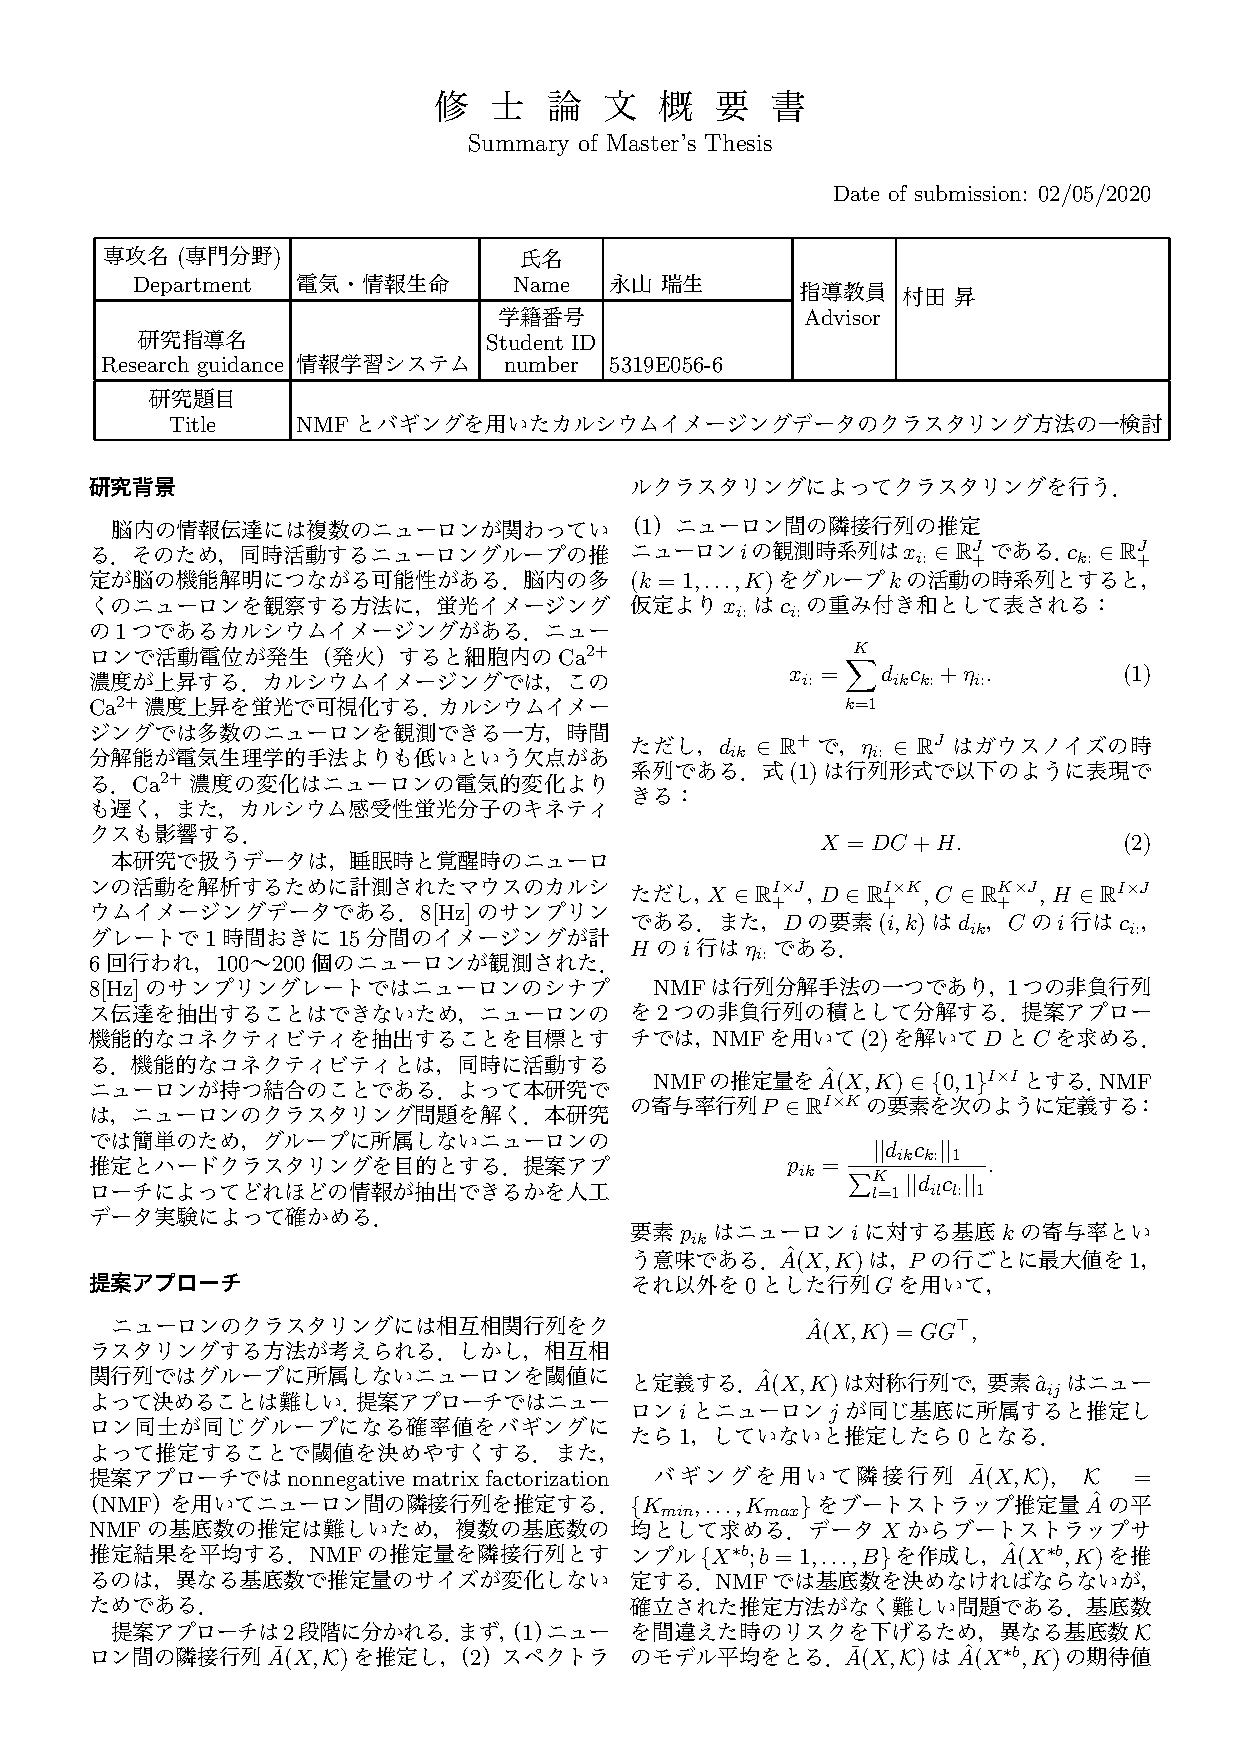
\includepdf[pages=-]{abstract.pdf}
%% ここまで
\tableofcontents

\mainmatter
%%% 以下本文
\chapter{序章}
\section{背景}
睡眠は脳によって制御されており\cite{Hobson2005},哺乳類にとって必要不可欠な生理現象である.
その重要性にも関わらず,睡眠について解明されていないことが多い.
その中でも,睡眠とはいかなる生物学的な状態か,という問いに対する明確な答えは未だない\cite{Kanda2016}.

哺乳類の睡眠状態は脳波によって定義される.
しかし,哺乳類以外は脳波を計測することができないためふるまいでしか評価できない.
そこで,ニューロンの活動から睡眠を新たに定義することができれば睡眠状態の解明に繋がると考えられる\cite{Kanda2020}.

脳内の情報伝達は複数個のニューロンによって行われている.
また,睡眠時には多数のニューロンが活動してある現象が見られることが知られている.
複数ニューロンの活動を解析することが重要である.

ニューロンの観察方法として,パッチクランプ法,細胞内記録法,細胞外記録法などの電気生理学的な手法が挙げられる.
これらの手法は十分な時間分解能かつ細胞レベルでニューロンを観察することができる.
しかし,電気生理学的な手法では観察できるニューロンの数は数十から多くても数百程度である.

より多くのニューロンを観察するために,蛍光イメージングの1つであるカルシウムイメージングという手法が用いられる.
ニューロンで活動電位が発生(発火)すると細胞内の$\text Ca^{2+}$濃度が上昇する.
カルシウムイメージングでは,この$\text Ca^{2+}$濃度上昇を蛍光で可視化する.
具体的には,$\text Ca^{2+}$と結合すると蛍光強度が変化する蛍光分子を細胞内に発現させておき,$\text Ca^{2+}$濃度を蛍光強度として蛍光顕微鏡で観察する.
蛍光イメージングを用いる利点として,(1)高い空間分解能,(2)広い観察範囲,(3)遺伝子工学と併用して興奮性/抑制性ニューロンの同定などをした上での観察ができることが挙げられる.
一方,時間分解能が電気生理学的手法よりも低いことが蛍光イメージングの欠点である.
$\text Ca^{2+}$濃度の変化はニューロンの電気的変化よりも遅く,また,カルシウム感受性蛍光分子のキネティクスも影響する.
さらに,カメラやレーザースキャンでのサンプリングレートは高くても100Hz程度であり,ニューロンの個々の発火を全て捉えるには不十分である.

本研究で扱うデータは,8Hzのサンプリングレートで観察された100〜200個のマウスのニューロンのカルシウムイメージングデータである.
本研究では,低い時間分解能のカルシウムイメージングデータからニューロンをクラスタリングし,人工データ実験を通してどの程度の情報が抽出できるかを確認する.

\section{カルシウムイメージングデータ}
本節では,カルシウムイメージングデータがどのようなデータなのかを説明し,どの程度の情報が取り出せるかを議論する.

ニューロンは1[ms]単位で活動電位が発生する(発火).
活動電位は細胞内外のイオン濃度が局所的に変化することによって生じる.
活動電位は細胞体から軸索を伝わり,シナプスを介して結合している別のニューロンに伝わる.
哺乳類の皮質ニューロンにおいて,ニューロンからニューロンへシナプスを介して活動電位が伝わるには数十[ms]かかる\cite{Izhikevich2004}.
このように活動電位を伝えることによってニューロン間で情報がやり取りされる.

ニューロンが他のニューロンとコネクションを持つ状態のことをコネクティビティという.
脳のコネクティビティには,anatomical connectivityとfunctional connectivityとeffective connectivityの3種類がある\cite{Sporns2007}.
Anatomical connectivityはニューロンが物理的に繋がっていることを指す.
Funcional connectivityを持つ2つのニューロンは活動に相関があり,機能が同じことを指す.
例えば,ある物を見た時,それに特異的に反応するニューロン群はfunctional connectivityを持つ.
Effective connectivityは,1つのニューロンから別のニューロンへ情報が伝わることを指す.
データによってどのコネクティビティの情報を取り出せるかは異なる.

1個1個のニューロンを1[ms]単位で計測できればニューロン全ての活動を計測できるが,そのような技術は存在しない.
ニューロンの計測方法には様々なものがあり,それぞれ計測可能な時間分解能と空間分解能が異なる.
計測方法別の分解能については\cite{Sejnowski2014}のFig 1が分かりやすい.
EEG,PET,fMRIは脳の一部のニューロンの活動によって生じた電位,血流,代謝量の変化を計測する.
これらの手法ではニューロン単位の計測は行えないが,脳全体を計測することができる.
電気生理学的な手法やカルシウムイメージングではニューロン単位で膜電位の変化やカルシウムイオン濃度の変化を計測する.
これらの手法ではニューロン1個1個を計測できるが脳全体を計測することはできない.

カルシウムイメージングとはニューロン内のカルシウムイオン濃度を可視化することでニューロンの活動を計測する手法である.
観察したい個体のニューロンにカルシウムイオンと結合する蛍光タンパク質を発現させると,細胞内のカルシウムイオン濃度に応じて蛍光強度が変化する.
ニューロンが発火するとカルシウムイオンが流入するため蛍光強度が上昇し,その後徐々に蛍光強度は減少する.
ニューロンを蛍光顕微鏡で観察することで\Figref{fig:imagingB}のような蛍光強度を反映した画像が得られる.
その画像から個々のニューロンの蛍光強度のデータを取得できる.
\begin{figure}[htbp]
	\centering
	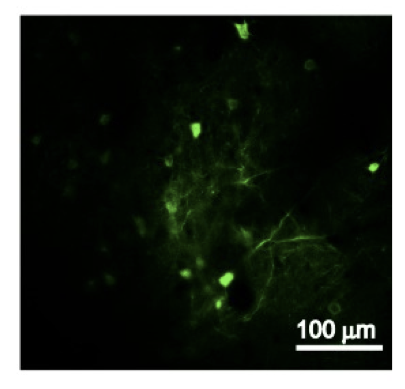
\includegraphics[width=0.5\hsize]{imagingB}
	\caption{カルシウムイメージングで観察できる画像の例.}
	\label{fig:imagingB}
\end{figure}

電気生理学的な手法と比べた時のカルシウムイメージングの利点として,ニューロンの位置情報が分かるため同じニューロンを複数回観察できることとより多くのニューロンの測定ができることが挙げられる.
また,ニューロンには興奮性ニューロンと抑制性ニューロンの二種類があり,カルシウムイメージングではこの種類を見分けることができる.
二種類の蛍光タンパク質を用いて,片方の蛍光タンパク質を抑制性ニューロンのみに発現させることで興奮性・抑制性が分かる.

カルシウムイメージングが電気生理学的な手法より劣る点として,時間分解能が挙げられる.
カルシウムイメージングのサンプリングレートは測定機器に限界があり\cite{Nakamura2003},通常1-50[Hz]程度である.
ニューロンの発火は約1[ms]で,シナプスを介して発火が伝わるのは40[ms]以内\cite{Bi1998}なので,ニューロンの発火を個別に観測することはできず,低いサンプリングレートでは発火の伝達も捉えることができない.
また,カルシウムイオン濃度の変化は発火のタイムスケールより長い.
発火後に蛍光強度が変化し始めるのは数[ms]後,蛍光強度がピークに達するのは数100[ms]後である.
一方,蛍光強度が元の値に戻るまでには,数100[ms]から数1000[ms]かかる\cite{Hira2018}.
また,蛍光タンパク質の性能によっても時間遅れが生じる.

本研究で扱うデータのサンプリングレートは8[Hz]で,シナプス伝達一つを見るには不十分である.
顕微鏡で観測すると活動電位が伝わる順番は分からなくなるため,カルシウムイメージングデータからはニューロンの活動の相関の情報しか得ることができない.
% また,脳の神経細胞はシナプスを3つか4つ介せば全て繋がると言われているため,局所的なネットワーク構造を考える必要はないと考えられる.
これより,このデータではニューロン間のシナプス伝達を推定するのではなく,機能的に同じニューロン,つまり同時に活動するニューロングループを推定する問題が適していると考えられる.
機能的に同じニューロンは,3つの脳のコネクティビティのうちfunctional connectivityで繋がっているニューロンを指す.

\section{関連研究}
\subsection{脳データの解析}
カルシウムイメージングは時間解像度が低く空間解像度が高いデータが取得できる手法である.
同じ特徴であるfMRIに対するデータの解析手法を紹介する.

fMRIデータの解析はmodel basedな手法とdata-drivenな手法がある\cite{Li2009}.
Model basedな手法はcross-correlation analysis (CCA)やcoherence analysis (CA)などが挙げられ,各指標に基づいて脳部位(ROI)の機能的な結合(前述のfunctional connectivity)を推定する.
CCAでは2つのROIの相関を使う.
CAでは,2つのROIの周波数ドメインでの相関を見る.
fMRIのBOLD信号の周期は10[s]ほどなので,0.1[Hz]以下の周波数ドメインでの相関を見る.
結合の有無は各指標の閾値で決めなければならない.
Data-drivenな手法は更に行列分解とクラスタリングに分けることができる.
行列分解にはprincinpal component analysis (PCA)やsingular value decomposition (SVD),independent component analysis (ICA)などが挙げられ,BOLD信号を複数の成分に分解することができる.
同じ成分の重みが大きいROIは結合があるとする.
ICAは成分数を事前に与える必要がある.
クラスタリングはfuzzy clustering analysis (FCA)やhierarchical clustering analysis (HCA)などがある.
クラスタリングではデータ間の距離を定義する必要がある.
FCAはあるROIが複数のクラスタに存在できるクラスタリング手法で,クラスタ数を事前に決める必要がある.
HCAはクラスタ数を決めずにROIやクラスタが近いか遠いかを見ることができる.

本研究では,行列分解手法の1つであるNMFを用いて隣接行列を推定する.
数理モデルを仮定すると,カルシウムイメージングデータにはICAやPCAよりNMFの方がデータに適している.

\subsection{カルシウムイメージングの解析例}
カルシウムイメージングデータの解析には二種類考えられる.
まずは,カルシウムイメージングデータからスパイクを推定し,そのスパイク列を解析する方法である.
Vogelsteinらは逐次モンテカルロ法を用いてカルシウムイメージングデータからスパイク推定を行なった\cite{Vogelstein2009}.
しかし,カルシウムイメージングデータでも低いサンプリングレートで計測されたデータではこの方法は使えない.

もう一つは,データから直接ニューロンの活動を解析する方法である.
Mishchenckoはベイズ推定を用いたニューロンの結合推定を行なった\cite{Mishchencko2011}.
しかし,カルシウムイメージングのサンプリングレートが30[Hz]以上でないと意味のある結合推定結果は得られないと報告している.
また,Stetterらはtransfer entropy(TE)を用いて培養された興奮性ニューロンの結合推定を行なった\cite{Stetter2012}.
この手法では,2つのニューロン間のTEを計算し,向きのあるエッジを推定している.
また,ニューロンのネットワーク構造を仮定した人工のカルシウムイメージングデータを作成し,推定精度を議論している.
しかし,本研究で扱うデータはサンプリングレートが低いため,向きの情報は取り出せない.
Ikegayaらは蛍光強度データの一次微分を閾値で切ることで発火のタイミングの情報を取り出し,テンプレートマッチングによってリアクチベーション現象を解析した\cite{Ikegaya2004}.
この研究では1[Hz]のデータからもリアクチベーション現象を確認できていた.
しかし,本研究ではニューロン集団を推定したいため,この方法はあまり適さない.

Molterらはカルシウムイメージングデータからニューロングループを抽出する方法を8つ人工データ実験と共に試した\cite{Molter2018}.
手法は大きく2つに分けられ,ニューロンペアの相関を見るものと,全てのニューロン活動の状態を見るものである.
前者では固有値分解によって相関行列を作成した後,ICAやPromax rotationによってグルーピングを行う.
後者では,ニューロンの活動からSVD,k-meansクラスタリング,スペクトラルクラスタリングなどを用いてグルーピングを行う.
後者の方法では,各グループの時間方向の活動を平均をとるなどして,グループの活動としていた.
人工データは,ニューロンをポアソン分布にしたがって発火させ,発火からカルシウムイメージングの観測データに変換していた.
同じグループに所属するニューロンは発火確率を同じ時間帯にあげることで表現していた.
用いられていた手法では,ニューロンが複数グループに所属する場合やグループに所属しない場合も対応ができる.
最も良いと結論づけられていた手法はICA-CSとSGCという手法だったが,どちらの手法も閾値などのパラメータを決めなければならない.

Ghandorらは学習に関係するニューロン(engram cell)群についてNMFを用いて解析を行った\cite{Ghandour2019}.
実験は複数セッションに分けて行われており,それぞれのセッションでNMFを用いてニューロングループとその活動に分解していた.
基底数はAICcで決めていた.
セッションごとに推定されたグループが近いかをcosine similarityで計った結果,engram cellではnon-engram cellよりも繰り返し活動するグループが多かった.
NMFによってニューロングループがどれほど抽出できるかは論じられていなかった.

\section{目的}
カルシウムイメージングデータは上述のように多くのニューロンを観測できる利点がある一方,時間分解能が低いという欠点を持つ.
本研究で扱うデータは低いサンプリングレートで観測されたデータである.
ニューロンは複数で活動することで情報伝達を行っており,睡眠時に多数のニューロンが同時に活動する現象も確認されている.
これより,本データでは同時に活動するニューロングループを推定して解析を行うことが適当である.

本研究の目的は,カルシウムイメージングデータから同時に活動するニューロングループを推定することである.
紹介した関連研究は,本研究で扱いたいデータのサンプリングレートでは使えないものや,パラメータを適切に決めなければならないものだった.
提案アプローチでは,数理モデルに基づいてNMFを用いてニューロンの隣接行列を推定し,スペクトラルクラスタリングを用いて隣接行列からクラスタリングを行う.
隣接行列はバギングを用いて,2つのニューロンが同じグループになる確率値をつける.
そのため,グループに所属しないニューロンの推定や,どれくらい結果を信用して良いのかがわかる.
その際も閾値を決めなければいけないが,確率値という分かりやすい指標のため,既存手法より簡単だと思われる.
NMF自体も基底数を事前に決めなければいけないが,大体の基底数を決めればその基底数周りの結果を平均することでパラメータによる結果の劇的な変化を抑えることができる.
また,人工データ実験によって提案アプローチがカルシウムイメージングデータからニューロングループの情報をどの程度取り出せるかを確かめる.

本論文の構成は以下の通りである.
第2章では本研究で使う手法の説明をする.
第3章では数理モデルを元にしたクラスタリングのアプローチを説明する.
第4章では人工データの作成方法と人工データ実験の結果,実データ解析の結果を述べる.
第5章で本研究をまとめる.
また,付録Aにカルシウムイメージングデータのために考案したNMFの制約を,付録BにNMFのモデルエビデンスの推定を試みた結果を載せる.

\chapter{準備}
本節では,提案アプローチで用いるNMF,バギング,スペクトラルクラスタリングについて説明する.
\section{NMF}

\section{バギング}

\section{スペクトラルクラスタリング}

\chapter{手法}
本章では検討した解析方法について述べる.
\section{解析のアプローチ}
\subsection{分解能の決定}
ニューロンの活動データの扱いには時間分解能と空間分解能の2つの側面から検討する必要がある.
時間分解能については,蛍光強度データをそのまま用いる,移動平均をとる,時間窓に区切るなどが考えられる.
空間分解能については,ニューロン1個を見る場合,2個を見る場合,複数を見る場合が考えられる.
手法によってどのレベルでデータを扱うかが異なる.
\Tabref{tab:methods}にカルシウムイメージングデータを解析する際に使えそうな手法を載せる.

\begin{table}[htb]
  \center
  \begin{tabular}{|c|cc|} \hline
    & 生データ & 時間窓で区切る \\ \hline
    ペアで見る & 時系列クラスタリング & glasso,類似度+クラスタリング\\
	  複数で見る & 行列分解 & ロジスティック回帰,時系列クラスタリング \\ \hline
  \end{tabular}
  \caption{カルシウムイメージングデータ解析に使えそうな手法}
  \label{tab:methods}
\end{table}

本論文では,データに対して仮説をおいて数理モデルを立てた上で,行列分解を用いることにする.

\section{モデル}
カルシウムイメージングデータを解析するに当たって,いくつかの仮説をおいた.
\\
\noindent \textbf{仮説 1}\\
グループが$K$個存在し,同じグループのニューロンは同時に活動する.
ニューロンは複数のグループに所属することができる.
観測時間内ではグループに属するニューロンは変化しない.\\
\textbf{仮説 2}\\
複数のグループが同時に活動する時,属するニューロンは被らない(ニューロンが属するグループは同時には活動しない).
\\

これらの仮説をもとに,数理モデルを構築する.
$c_k$, ($k=1,\dots,K$)をグループ$k$の活動の時系列とする.

ニューロン$i$の観測時系列を$x_i$とおき,$c_k$の重み付け和で表す:
\begin{equation}
  x_i = \sum_{k=1}^K d_{ik} c_k + \eta_i.
  \label{eq:x}
\end{equation}
$\eta_i$はガウスノイズである.
カルシウムイメージングのノイズはポアソン分布に従う光子ノイズであるが,光子数が多い場合はガウス分布で近似できる~\cite{Sjulson2007}.

$\mathbb{R}_+$を非負の実数の集合とする.
\Eqref{eq:x}は行列形式で以下のように表現できる:
\begin{eqnarray}
  Y &=& DC, \\
  X &=& Y + H.
  \label{model_matrix}
\end{eqnarray}
ただし,$X \in \mathbb{R}_+^{N \times T}$, $D \in \mathbb{R}_+^{N \times K}$, $C \in \mathbb{R}_+^{K \times T}$, and $H \in \mathbb{R}^{N \times T}$である.
また,$X$の行は$x_i$,$D$の要素$(i,k)$は$d_{ik}$,$C$の行は$c_i$,$H$の行は$\eta_i$である.
これ以降,行列$A$の$i$行を$A_{i:}$,$j$列を$A_{:j}$,$(i,j)$要素を$A_{ij}$と表記する.

解くべき問題は$D$と$C$を推定することである.

ニューロンがどのグループに所属しているかを評価する方法として,寄与率を導入する.
ニューロン$i$に対するループ$k$の寄与率を以下のように定義する:
\begin{equation}
	\frac{|| d_{ik} c_k ||_1}{\sum_{l=1}^K || d_{il} c_l ||_1}.
  \label{eq:pov}
\end{equation}
寄与率が高いグループにニューロン$i$が所属すると考えることにする.

\chapter{人工データ実験}
\section{シミュレーション}
ニューロン集団のカルシウムイメージングデータをシミュレーションによって作り,解析手法を評価する.
シミュレーションでは1)ニューロンのネットワーク構造を作成し,2)スパイクのシミュレーションを行い,3)蛍光強度の観測データに変換する.
\subsection{ネットワーク構造}
ニューロンのネットワーク構造にはsmall world network\cite{Watts1998}を用いる.
Small world networkはノード数,張り替え確率,初期次数を決めることによってネットワークを作成するアルゴリズムである.
初期次数は,ニューロンが平均何個のニューロンとシナプス結合を持つかという変数である.
張り替え確率は,初期次数によって作成された規則的なグラフのエッジをランダムに張り替える確率である.
そのため,エッジのうち何割が遠くのニューロンとつながっているかを表す変数である.

実際のニューロンをsmall world networkによって表すために,初期次数と張り替え確率を実データから決める.
今回はこの値はニューロンのコネクションの割合と相互のコネクションの割合から決める.
興奮性ニューロン同士の6.7\%であり,そのうち双方向のコネクションの割合は24\%である\cite{}.
成熟したマウスの抑制性ニューロンと興奮性ニューロンのコネクションの割合は不明だが,興奮性ニューロンから抑制性ニューロンへのコネクティビティと抑制性ニューロンから興奮性ニューロンへのコネクティビティはどちらも78\%であった\cite{Holmgren2003}.
成熟したマウスではより少ないと思われるが,データが見つからなかったため,40\%とした.
相互のコネクションの割合がランダムにエッジを作るよりも高いのは,近いニューロンにコネクションが作られやすいからだと考えられる.
これらのデータを実現するように初期次数と張り替え確率を調整した.
また,抑制性ニューロン同士のコネクティビティは分からないため,興奮性と同じにしている.
\subsection{スパイクシミュレーション}
スパイクのシミュレーションにIzhikevichモデル~\cite{Izhikevich2003}を用いる.
このモデルはHodgikin-Huxleyモデルをもとにしており,計算コストが低い.
このモデルにはニューロンごとに4つのパラメータを設定する必要があり,そのパラメータでニューロンを特徴づける.
本論文では興奮性ニューロンにはregular spiking neurons,抑制性ニューロンにはfast spiking neuronsを用いる.
それらのパラメータを~\Tabref{tab:parameter1}に示す.
ただし,$r_e$と$r_i$は0から1の一様分布に従う確率変数である.

\begin{table}[htb]
  \center
  \begin{tabular}{|c|cccc|} \hline
    ニューロンの種類 & a & b & c & d \\ \hline
    興奮性ニューロン & 0.02 & 0.2 & $-65 + 15 r_e^2$ & $8 - 6r_e^2$ \\
    抑制性ニューロン & $0.02 + 0.08r_i$ & $0.25 - 0.05 r_i$ & -65 & 2 \\ \hline
  \end{tabular}
  \caption{Izhikevichモデルのパラメータ}
  \label{tab:parameter1}
\end{table}

ニューロン間でどれだけシナプス伝達が行われるかも決めなければならない.
これは隣接行列で表すことができる.
隣接行列の$(i,j)$要素は,ニューロン$j$が発火した際にどれくらいの電位がニューロン$j$からニューロン$i$に伝わるかを表す.
興奮性ニューロンからの電位は0から0.5の一様分布からサンプルし,抑制性ニューロンからの電位は-2から0の一様分布からサンプルする.

ニューロンには観測範囲外からの入力がある(以降,外部入力とする).
そのため,シミュレーション中も外部からの電位を乱数としてニューロンの電位に足す.
本論文では,ニューロンの活動も外部入力の大きさで表現する.
活動していない興奮性ニューロンと抑制性ニューロンにはそれぞれ,$\mathcal{N}(0,5)$と$\mathcal{N}(0,2)$に従う乱数を足す.
活動している興奮性ニューロンと抑制性ニューロンにはそれぞれ,$\mathcal{N}(1,5)$と$\mathcal{N}(0.4,2)$に従う乱数を足す.
これらを\Tabref{tab:parameter3}に示す.
活動していないニューロンへの外部入力は\cite{Izhikevich2003}で用いられていたものを採用した.

\begin{table}[htb]
  \center
  \begin{tabular}{|c|cc|} \hline
    ニューロンの種類 & 活動時の外部入力 & 活動していない時の外部入力 \\ \hline
		興奮性ニューロン & $\mathcal{N}(1,5)$ & $\mathcal{N}(0, 5)$ \\
		抑制性ニューロン & $\mathcal{N}(0.4, 2)$ & $\mathcal{N}(0, 2)$ \\ \hline
  \end{tabular}
  \caption{シミュレーションに用いる外部入力の値}
  \label{tab:parameter3}
\end{table}

本論文では同時に活動するニューロンを推定するのが目的の1つである.
ある時間帯にあるニューロングループが活動する時,そのニューロングループには平均値を上げた外部入力を足し,それ以外のニューロンには平均$0$の外部入力を足す.
こうすることで,ニューロングループの活動のみ上がる(つまり蛍光強度が上がる).
実際の脳でもこのように外部からの入力によってニューロンの活動を制御していると考えられる.
あるニューロングループを活動させるには,そのグループのハブとなるニューロンにのみ強い外部入力を与える方法も考えられるが今回は採用しない.
なぜなら,ネットワーク構造をかなり工夫しないと実現できないためである.

\subsection{カルシウムイメージングモデル}
スパイクデータからカルシウムイオン濃度を計算する~\cite{Vogelstein2009}のモデルを用いる:
\begin{equation}
  [Ca^{2+}]_{i,t} - [Ca^{2+}]_{i,t-1} = - \frac{\Delta}{\tau}([Ca^{2+}]_{i,t-1} - [Ca^{2+}]_b) + An_{i,t} + \sigma_c \sqrt{\Delta} \epsilon_{i,t},
  \label{eq:calcium}
\end{equation}
ただし,$[Ca^{2+}]_{i,t}$をニューロン$i$の時刻$t$でのカルシウムイオン濃度,$[Ca^{2+}]_b$をカルシウムイオン濃度のベースライン,$\Delta$を時間幅,$\tau$は時定数,$A$は1つのスパイクでのカルシウムイオン濃度の上がり幅,$n_{i,t} \in \{0,1\}$はニューロン$i$の時刻$t$でのスパイク,$\sigma_c$はノイズの分散,$\epsilon_{i,t}$は標準正規分布に従う確率変数である.
この人工データではsaturationは考えないこととする.

次に,同論文のモデルを使ってカルシウムイオン濃度$[Ca^{2+}]_{i,t}$をカルシウムイメージングで計測される蛍光強度$F_{i,t}$に変換する:
\begin{equation}
	F_{i,t} = \alpha[Ca^{2+}]_{i,t} + \beta + \sigma_F \epsilon_{i,t},
  \label{eq:intensity}
\end{equation}
$\alpha$は強度,$\beta$はバイアス,$\sigma_F$はノイズの分散である.

\Tabref{tab:parameter2}に使用したパラメータを示す.

\begin{table}[htb]
  \center
  \begin{tabular}{|cccccccc|} \hline
    $[Ca^{2+}]_b$ & $\Delta$ & $\tau$ & $A$ & $\sigma_c$ & $\alpha$ & $\beta$ & $\sigma_F$ \\ \hline
    0.1 & 0.001 & 0.5 & 5.0 & 1.0 & 1.0 & 0 & 1.0 \\ \hline
  \end{tabular}
  \caption{カルシウムイメージングモデルでのパラメータ}
  \label{tab:parameter2}
\end{table}

\subsection{観測モデル}
実データは8 Hzでサンプリングされたデータなので,シミュレーションした蛍光強度を8 Hzで足し合わせる:
\begin{equation}
  x_{i,t'} = \sum_{t=1}^{125} F_{i,t},
  \label{eq:observation}
\end{equation}
ここで,$t'$はサンプリング後の時刻を表す.

上記の方法で作成した人工データ時系列と観測時系列をそれぞれ\Figref{fig:art}と\Figref{fig:dat}に示す.
\begin{figure}[htbp]
    \begin{minipage}{0.5\hsize}
			\begin{center}
					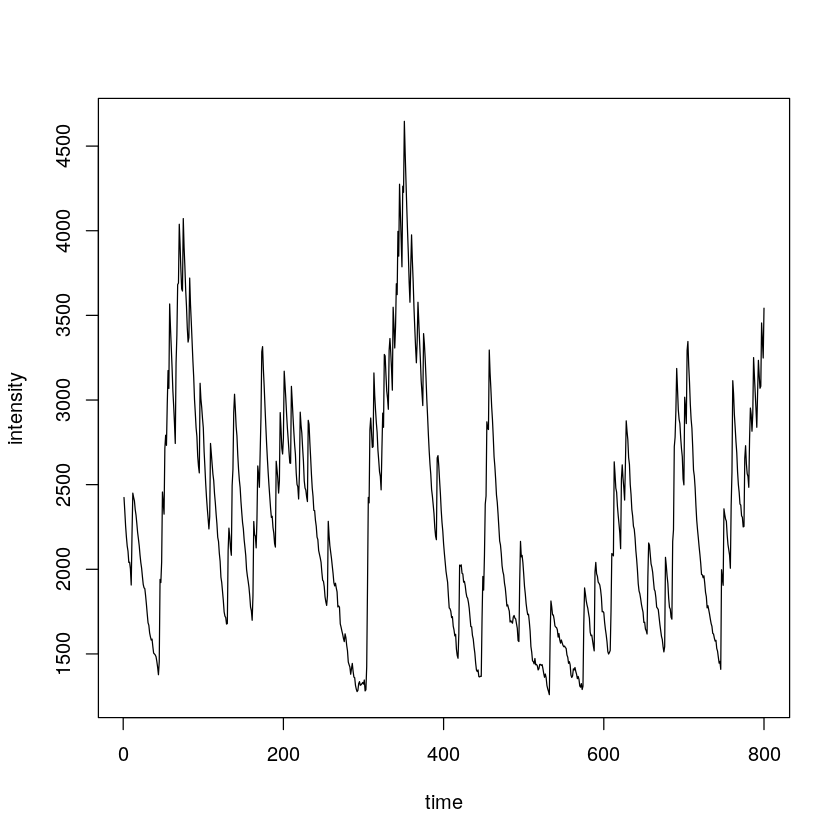
\includegraphics[width=\hsize]{artificial_data}
					\caption{1つのニューロンの人工時系列.}
					\label{fig:art}
			\end{center}
		\end{minipage}
    \begin{minipage}{0.5\hsize}
			\begin{center}
					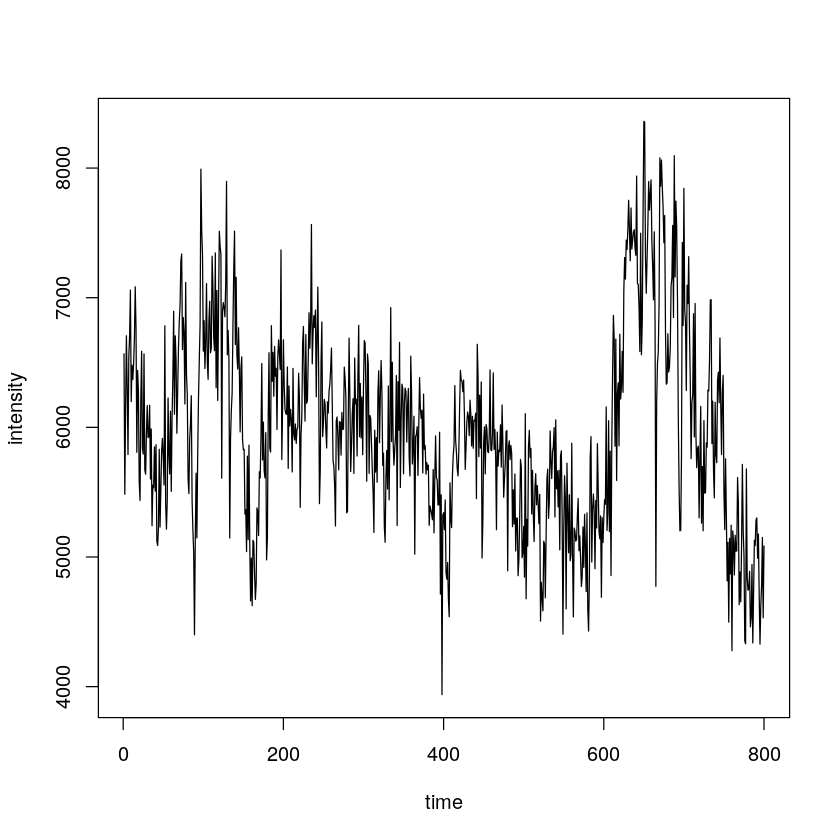
\includegraphics[width=\hsize]{real_data}
					\caption{1つのニューロンの観測時系列.}
					\label{fig:dat}
			\end{center}
		\end{minipage}
\end{figure}

\section{$A$の推定に関する結果}
\subsection{設定}
人工データは4種類作成した.
\begin{enumerate}
  \item ニューロンは1つのグループに必ず所属し,近いニューロン同士がグループとなっている
  \item ニューロンは1つのグループに必ず所属し,グループは近さに関係なくランダムに形成される
  \item ニューロンは1つか2つのグループに必ず所属し,同じニューロンが所属しているグループ同士の活動は被らない
\end{enumerate}
800個の興奮性ニューロンと200個の抑制性ニューロンについてシミュレーションを行った.
1つのグループに所属するニューロン数は50〜200個とした.
グループが活動する時間は5sごとに変えた.
シミュレーション時間は470sで,そのうちの10sは安定のため解析から除外した.

\subsection{$A$の一意性}
前章で述べた通り,NMFには一意性がないため$A$にも一意性がない.
1つの人工データについて初期値を変化させてNMFを行うと推定される$A$は同じではない.
$A$の上三角の要素について$1$と推定された頻度を調べる.
収束性と前章で述べたように寄与率が$D$の空間で取りうる値の範囲を狭めるため,$C$の行和を1とする制約を入れている.
$X$に正規化を加えなかった結果を\Figref{fig:without_scale_A}に,$X$に行和$1$の正規化を加えた結果を\Figref{fig:with_scale_A}に示す.
$X$に行和$1$の正規化を加えると,$D$の自由度は下がる.

\begin{figure}[htbp]
    \begin{minipage}{0.5\hsize}
			\begin{center}
					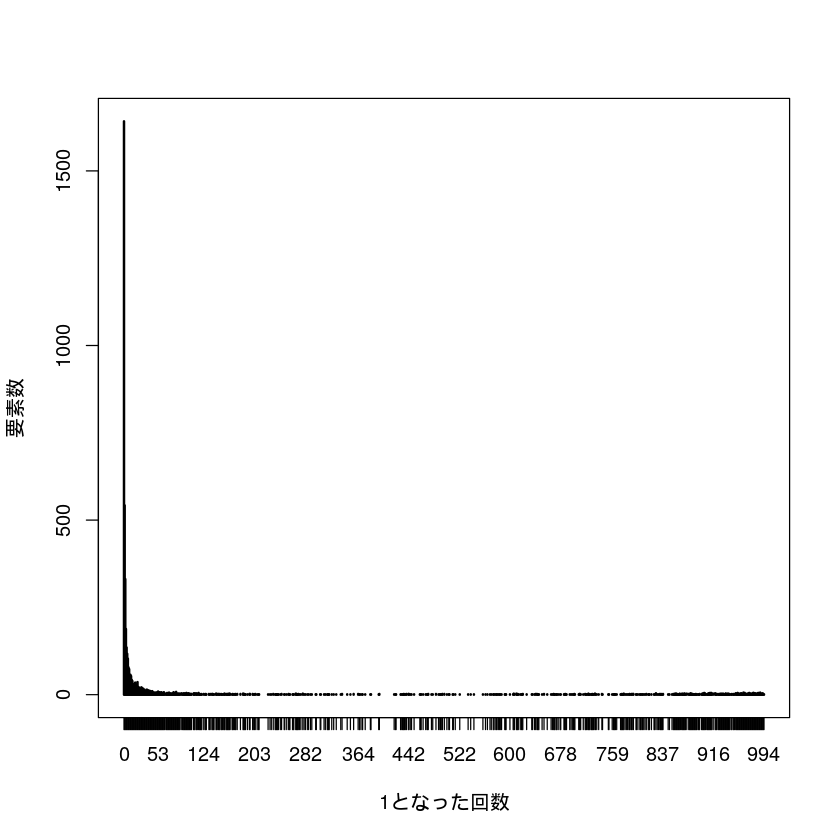
\includegraphics[width=\hsize]{without_scale_A}
					\caption{$X$を正規化せずに初期値を1000回変化させてNMFから$A$を推定し,各要素について$1$と推定された頻度をプロットした.}
					\label{fig:without_scale_A}
			\end{center}
		\end{minipage}
    \begin{minipage}{0.5\hsize}
			\begin{center}
					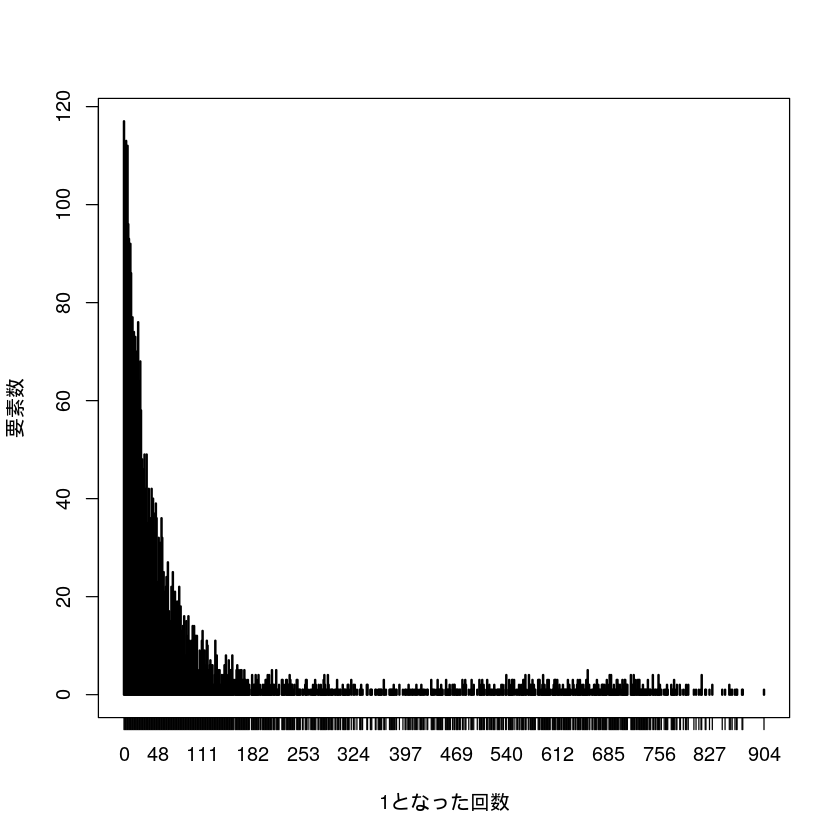
\includegraphics[width=\hsize]{with_scale_A}
					\caption{$X$を行和$1$で正規化して初期値を1000回変化させてNMFから$A$を推定し,各要素について$1$と推定された頻度をプロットした.}
					\label{fig:with_scale_A}
			\end{center}
		\end{minipage}
\end{figure}

$A$に一意性がある場合は,ある$A$の要素が$1$と推定される回数は$0$か$1000$になる.
結果より,そうなっていないので$A$に一意性がないのがわかる.
また,\Figref{fig:with_scale_A}より$X$を正規化した方がよりばらつきが大きくなっているのがわかる.
これは,正規化をしない方が$X$の中の大きな値に推定が引っ張られ,同じ局所解に落ちやすくなっているからだと考えられる.
また,この正規化の仕方は物理的には,ある期間にニューロンの活動の総和が一定であるという意味をもつ.
実際はそうではないので,今回の正規化の仕方はこの実験のみに留めておく.

\subsection{手法の比較}
NMF,PCA,ICA,logistic regression,glassoの性能の比較を行った.
Logistic regressionとglassoについては筆者の卒論を参照されたい.
どちらも時間窓をスライドさせてネットワークを行う.
今回の実験では時間窓を40,スライド幅を20とした.
Glassoのハイパーパラメータを$\rho = 0.3$とした.
一回でもエッジが張られたニューロン同士は同じグループとして推定量$A$と同じ行列を作成した.

PCAとICAはNMFと同じく一般化線形成分分析の手法\cite{Cichocki2009}である.
PCAとICAでは$D$に相当する行列でNMFと同じく推定量$A$を作成する.

2のタイプについて100種類のデータを生成し,$A$を閾値$0.5$で切って${0,1}^{I \times I}$の行列にした時のF1 scoreを比較した.
\begin{figure}[htbp]
    \begin{center}
        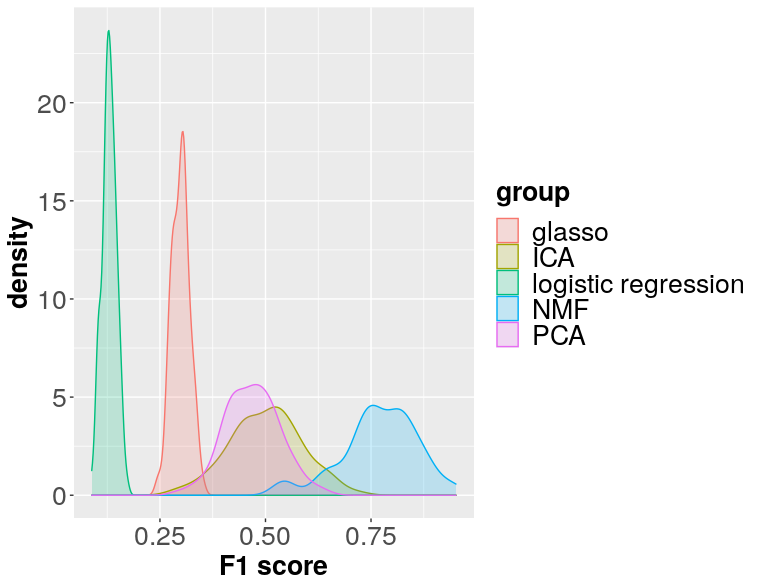
\includegraphics[width=0.5\linewidth]{compare-models}
        \caption{NMF,PCA,ICA,logistic regression,glassoのF1 scoreの密度分布}
        \label{fig:compare-models}
    \end{center}
\end{figure}
\Figref{fig:compare-models}より,NMFの精度が最も高いことが分かる.
NMFの非負制約がデータに合っているためだと思われる.
Glassoとlogistic regressionについてはニューロングループを推定するという実験設定はやや不利で合った.
各窓ごとのニューロンネットワークの活動を反映している可能性があるので悪い手法とはいえない.

% \subsection{推定へのネットワーク構造の影響}
% グループ推定へのネットワーク構造の影響を調べるために,1と2のネットワーク構造とグループについて100種類のデータを生成し,NMFの推定精度の比較を行った.
% 人工データは,近いニューロンほどつながりやすい性質をもつので,1の人工データの方がニューロン同士が同期して活動しやすいと思われる.
% ここで,2つのニューロンが同期するとは,一方のニューロンが発火してからごく短い間にもう一方のニューロンが発火する状態が続くことである.
% 実験結果を\Figref{fig:same-exc}~\ref{fig:diff-inh}に示す.
% \begin{figure}[htbp]
%     \begin{center}
%         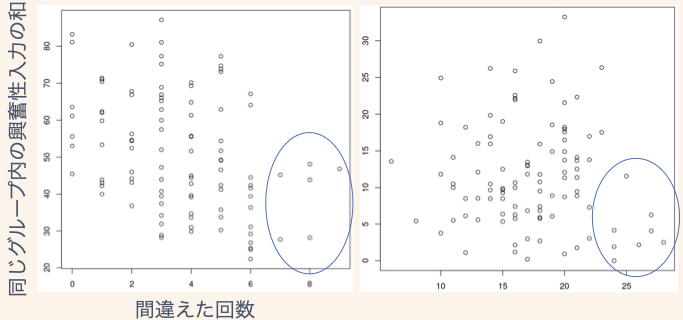
\includegraphics[width=\linewidth]{same-exc}
%         \caption{データ1と2について,ニューロンごとの間違えた回数と同じグループからの興奮性入力の和の関係}
%         \label{fig:same-exc}
%     \end{center}
% \end{figure}
% \begin{figure}[htbp]
%     \begin{center}
%       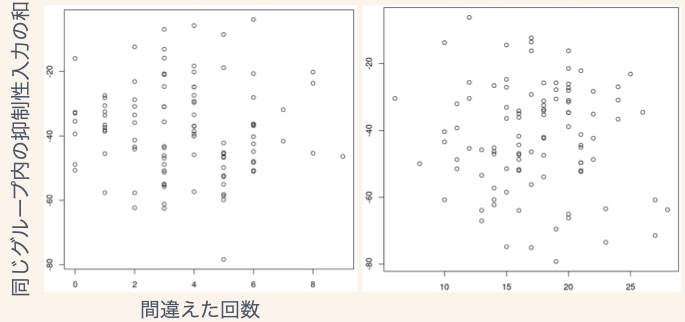
\includegraphics[width=\linewidth]{same-inh}
%         \caption{データ1と2について,ニューロンごとの間違えた回数と同じグループからの抑制性入力の和の関係}
%         \label{fig:same-inh}
%     \end{center}
% \end{figure}
% \begin{figure}[htbp]
%     \begin{center}
%         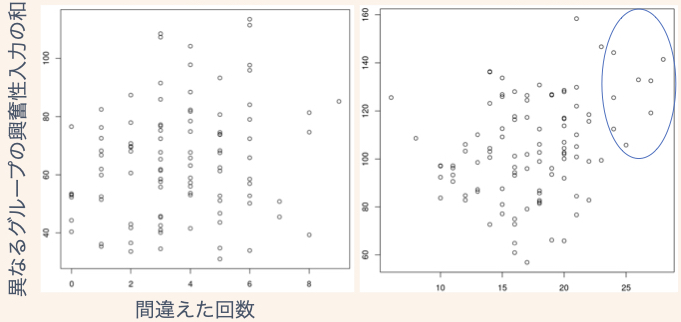
\includegraphics[width=\linewidth]{diff-exc}
%         \caption{データ1と2について,ニューロンごとの間違えた回数と異なるグループからの興奮性入力の和の関係}
%         \label{fig:diff-exc}
%     \end{center}
% \end{figure}
% \begin{figure}[htbp]
%     \begin{center}
%         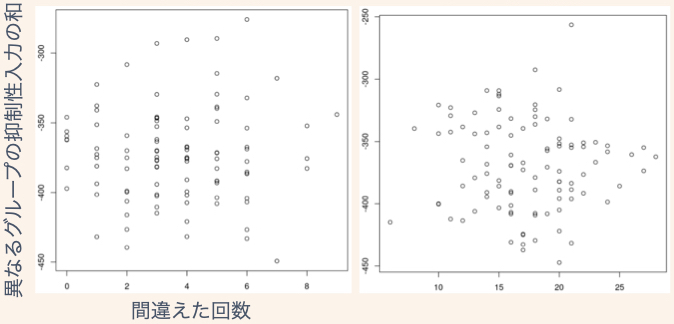
\includegraphics[width=\linewidth]{diff-inh}
%         \caption{データ1と2について,ニューロンごとの間違えた回数と異なるグループからの興奮性入力の和の関係}
%         \label{fig:diff-inh}
%     \end{center}
% \end{figure}
% \Figref{fig:same-inh},\Figref{fig:diff-inh}より,抑制性の入力は間違える回数には影響しないと思われる.
% \Figref{fig:same-exc}より,同じグループからの興奮性入力が小さいと間違えやすいと言える.
% \Figref{fig:diff-exc}より,データ2で間違える回数が多かったニューロンは異なるグループからの興奮性入力が大きかった.
% データ2ではデータ1よりも近いニューロンが異なるグループに所属する割合が多い.
% そのため,異なるグループからの興奮性入力と間違える回数の関係が強く出たと思われる.
% 
% 他にも推定へのネットワーク構造の影響の調査を試みたが,はっきりとした結果は得られなかった.

\subsection{2グループに所属するとき}
推定精度を出す.
そして被り率も出す.

\subsection{モデル平均の有用性}
バギングの有用性を確認するために各人工データについて,1回NMFを行った結果,30回初期値を変えた結果,30回ブートストラップした結果のF1 scoreを~\Figref{fig:once-init-boot}に示す.
なお,NMFは20回初期値を変化させて再構成ごさが最小となる結果を1回の結果として用いた.
\begin{figure}[htbp]
    \begin{minipage}{0.5\hsize}
			\begin{center}
					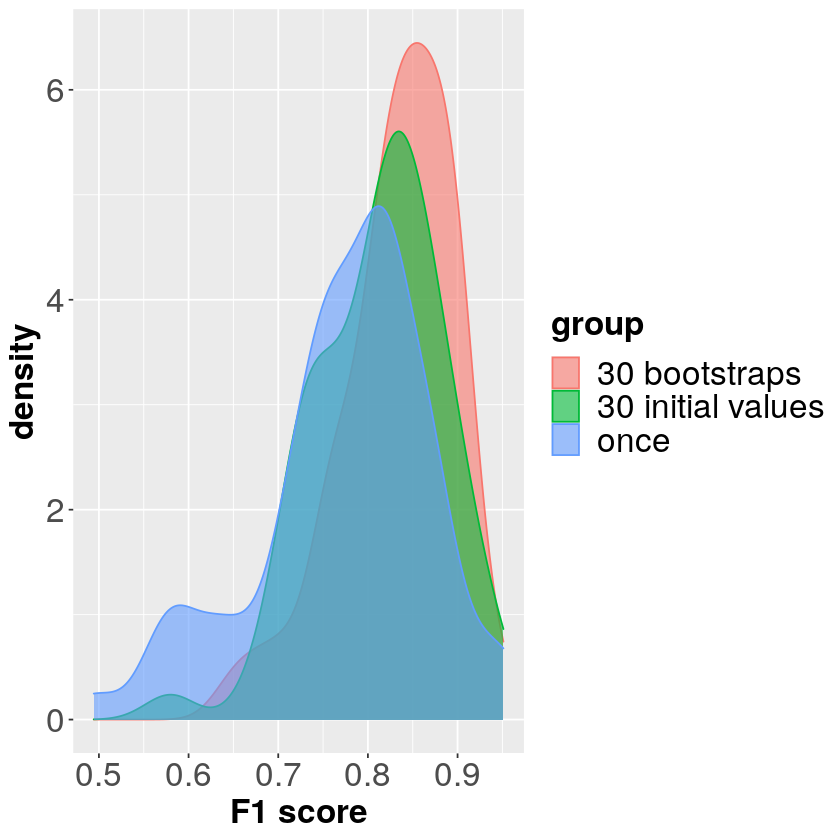
\includegraphics[width=\hsize]{once-init-boot}
					\caption{NMFを1回行った時の$A$,30回初期値を変えた$A$の平均,30回ブートストラップを行った$A$の平均それぞれのF1 scoreの分布.}
					\label{fig:once-init-boot}
			\end{center}
		\end{minipage}
    \begin{minipage}{0.5\hsize}
			\begin{center}
					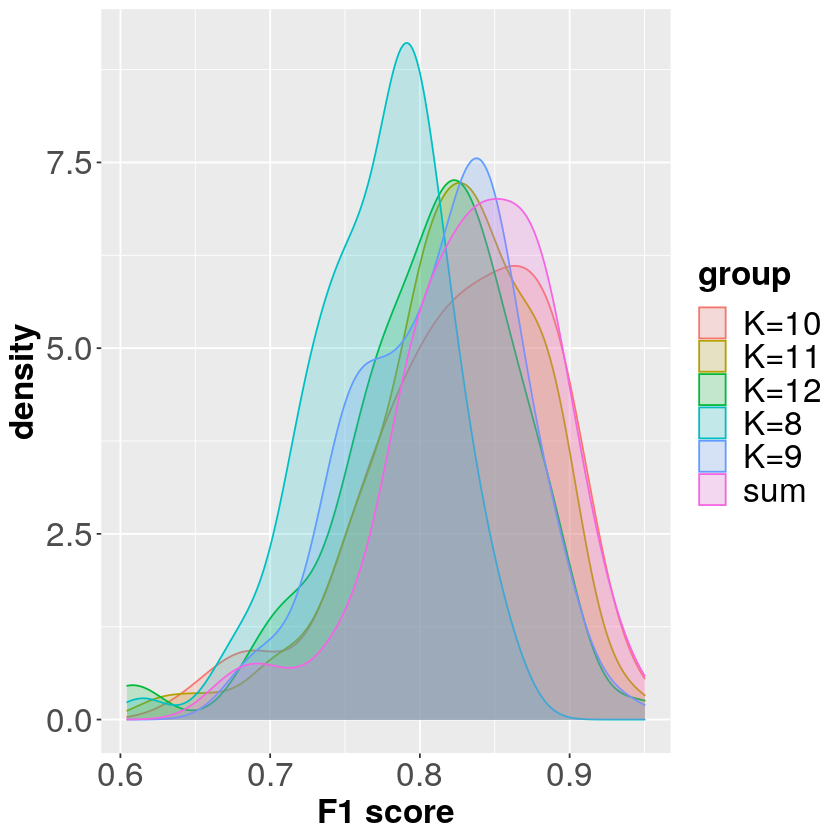
\includegraphics[width=\hsize]{f1all}
					\caption{基底数ごとにブートストラップを行った時の$A$のF1 scoreと全ての$A$の平均をとった時のF1 scoreの分布.}
					\label{fig:f1all}
			\end{center}
		\end{minipage}
\end{figure}
\Figref{fig:once-init-boot}より,ブートストラップを行った方が精度がよくなることがわかる.

基底数別に推定された$A$の平均をとった時のF1 scoreを~\Figref{fig:f1all}に示す.
これより,真の基底数周りの$A$の平均をとることである程度の精度は保たれることがわかる.

\subsection{NMFの基底数}
NMFの基底数を決める方法をいくつか試した.
人工データ86個についてBrunetらとUbrauらの方法で基底数を決めた時に各基底数が何回選ばれるかを~\Figref{fig:cophenetic}.\Figref{fig:uoi}に示す.
Brunetらの方法では真の基底数10に近い基底数が選ばれているが,Ubaruらの方法では小さい基底数が選ばれる傾向にあった.

また,1つの人工データについてAICとAICcを計算した結果を~\Figref{fig:aic},\Figref{fig:aicc}に示す.
どちらも基底数が大きくなるごとに減少する傾向があった.
他の人工データについても同様の結果であった.

\begin{figure}[htbp]
    \begin{minipage}{0.5\hsize}
        \begin{center}
            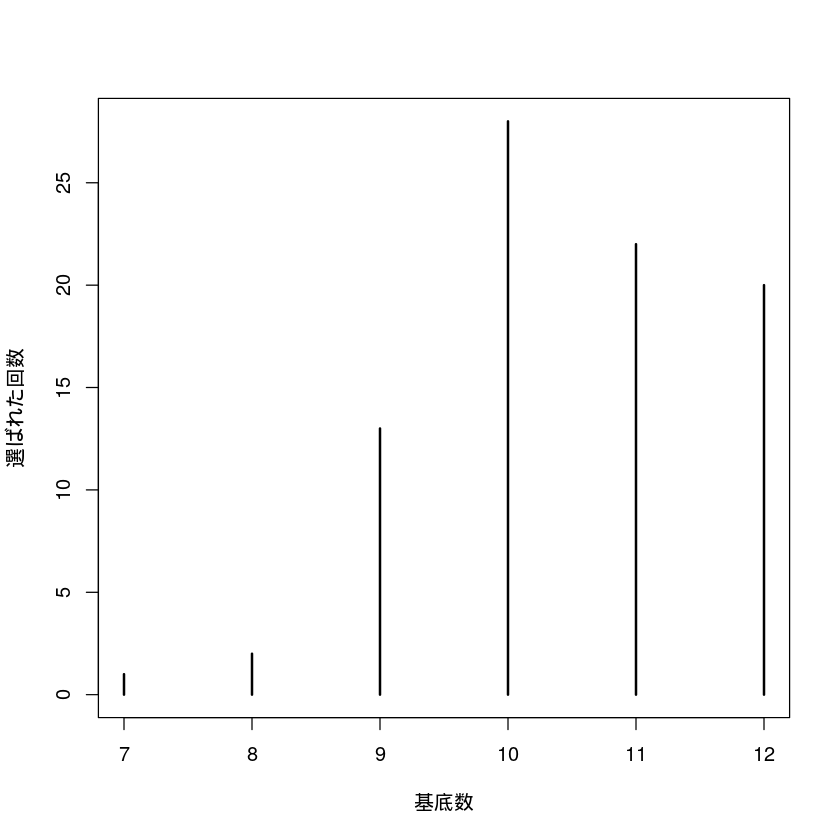
\includegraphics[width=\hsize]{cophenetic}
						\caption{Brunetらの方法で基底数を決めた時に各基底数が選ばれた回数(真の基底数は10).}
            \label{fig:cophenetic}
        \end{center}
    \end{minipage}
    \begin{minipage}{0.5\hsize}
        \begin{center}
            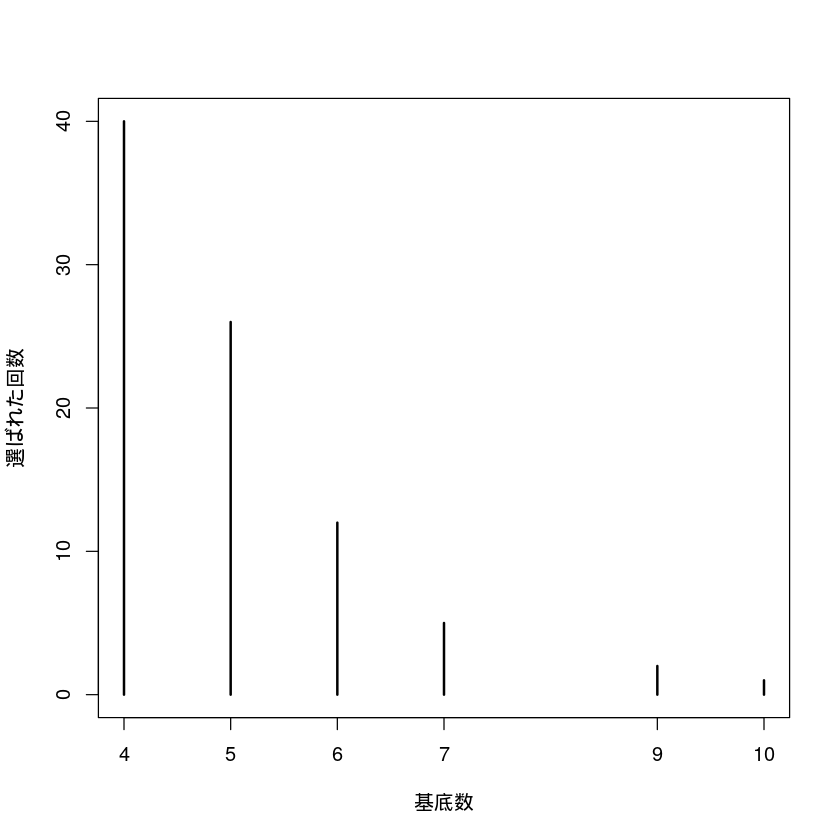
\includegraphics[width=\hsize]{uoi}
						\caption{Ubaruらの方法で基底数を決めた時に各基底数が選ばれた回数(真の基底数は10).}
            \label{fig:uoi}
        \end{center}
    \end{minipage}
\end{figure}
\begin{figure}[htbp]
    \begin{minipage}{0.5\hsize}
        \begin{center}
            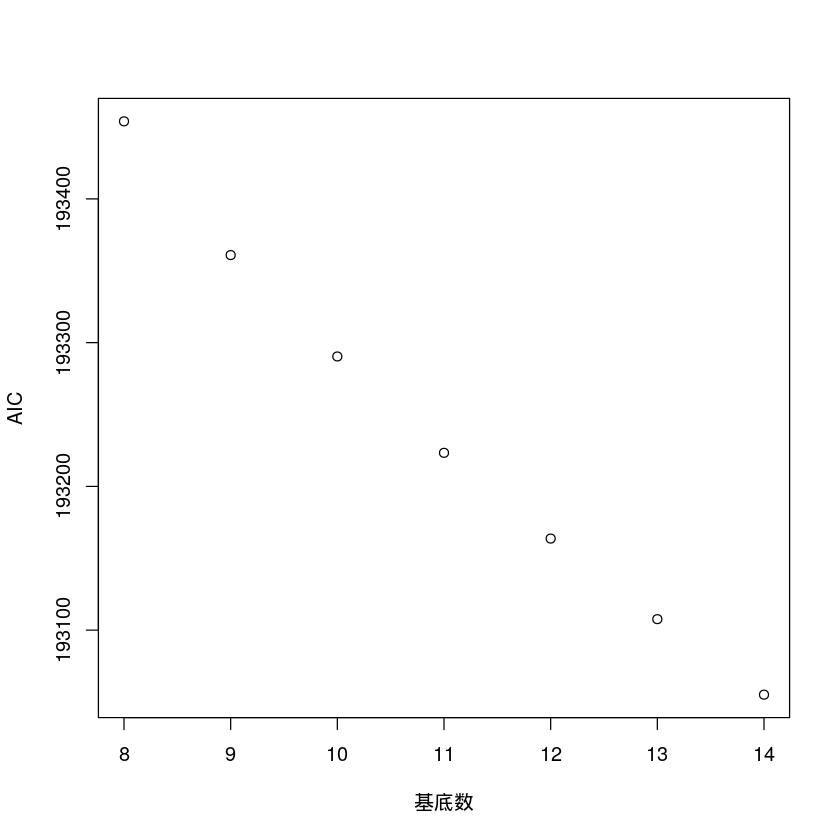
\includegraphics[width=\hsize]{aic}
						\caption{あるデータについてAICを計算した時の結果.}
            \label{fig:aic}
        \end{center}
    \end{minipage}
    \begin{minipage}{0.5\hsize}
        \begin{center}
						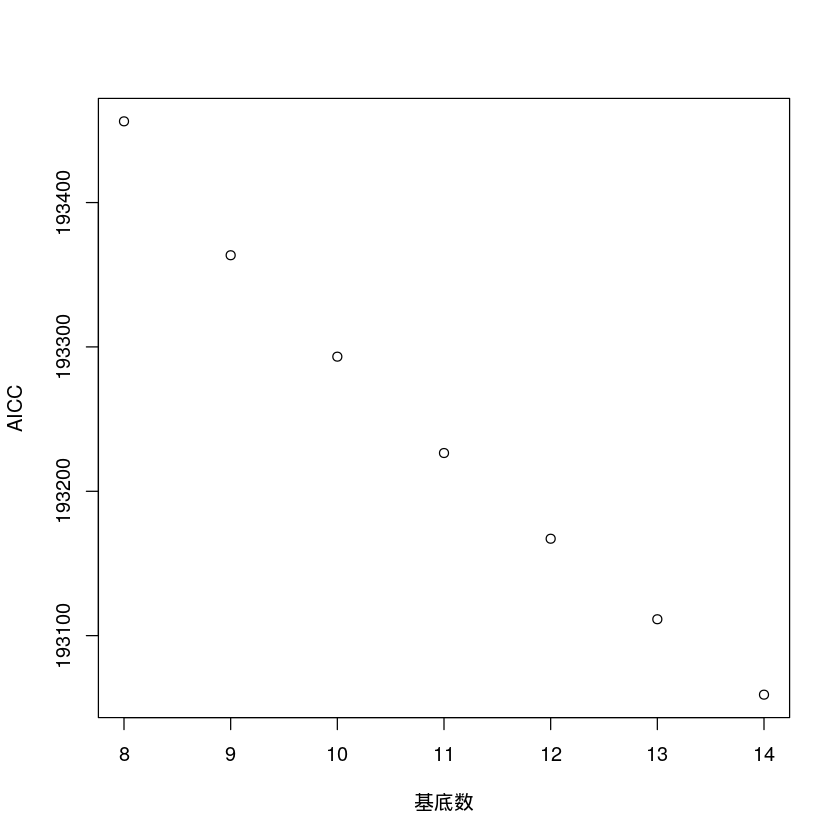
\includegraphics[width=\hsize]{aicc}
						\caption{あるデータについてAICc\cite{Symonds2011}を計算した時の結果.}
            \label{fig:aicc}
        \end{center}
    \end{minipage}
\end{figure}

\subsection{}

\section{$A$のクラスタリングに関する結果}
\subsection{クラスタ数の決定}
スペクトラルクラスタリングでクラスタ数を決定する方法はいくつかあるが,その中でも小さい固有値を見る方法と,Gap統計量を用いた方法を試す.
$A$と比較する類似度行列として,データの相互相関行列と分散共分散行列を用いる.

\chapter{実データ解析}
本章では実データを解析する.
本章では「NMF1回の結果」は「初期値を100回変えてNMFを行い目的関数が最小となった結果」とする.

\section{実データ}
本研究で用いるデータは筑波大学の柳沢研究所で計測されたカルシウムイメージングデータである.
本データは,2光子多細胞カルシウムイメージングによって1匹のマウスの大脳皮質1次運動野第2・3層のニューロンのイメージング画像を得た後,人手でROIがつけられ,ニューロンごとの数値データに直されたものである.
1時間おきに15分間のイメージングが計6回行われ,各イメージングのサンプリングレートは8[Hz]である.
このサンプリングレートは使用された機器の最大のものである.
用いられた蛍光タンパク質はGCaMP6sである.
実験系は\Figref{fig:imaging}(A)の系で行われた\cite{Kanda2016}.
観測されたニューロン数は154であった.
時間方向には4[s]ごとのマウスの状態(wake, REM, NREM)のラベルが付いており,ニューロンごとに興奮性か抑制性のラベルがついている.
\Figref{fig:wholedata}にニューロン3つの時系列と時系列方向についているラベル(wake,NREM,REM)を示す.

\begin{figure}[htbp]
    \begin{center}
				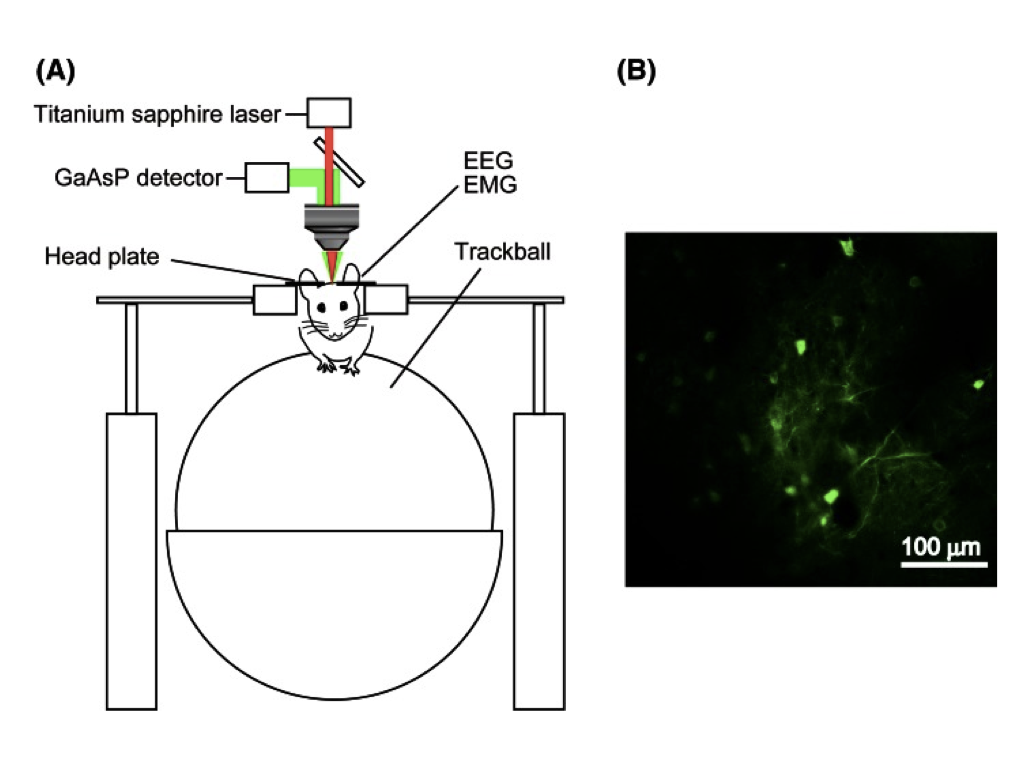
\includegraphics[width=0.8\linewidth]{imaging}
				\caption{(A)カルシウムイメージングの測定系.マウスは頭を固定されたままボールの上で活動することができる.(B)カルシウムイメージング画像.}
        \label{fig:imaging}
    \end{center}
\end{figure}

\begin{figure}[htbp]
	\begin{center}
		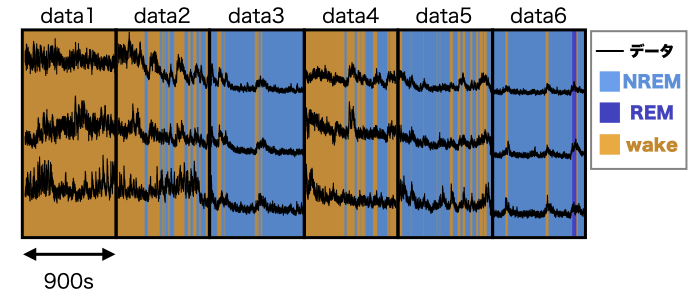
\includegraphics[width=\hsize]{datawhole}
	\end{center}
	\label{fig:wholedata}
\end{figure}

\section{実験設定}
6回計測されたデータそれぞれについてクラスタリングを行う.
NMFを一回行,それを最尤推定の結果とする.
最尤推定結果からBICを計算し,目視で基底数の範囲を決める.
範囲内の基底数について100回ブートストラップを行い,$\bar{A}$を求める.
固有値ギャップを算出し,スペクトラルクラスタリングを行う.

\section{結果}
推定されたクラスタを\Figref{fig:real-clst}に示す.

\begin{figure}[htbp]
    \begin{minipage}{0.32\hsize}
			\begin{center}
					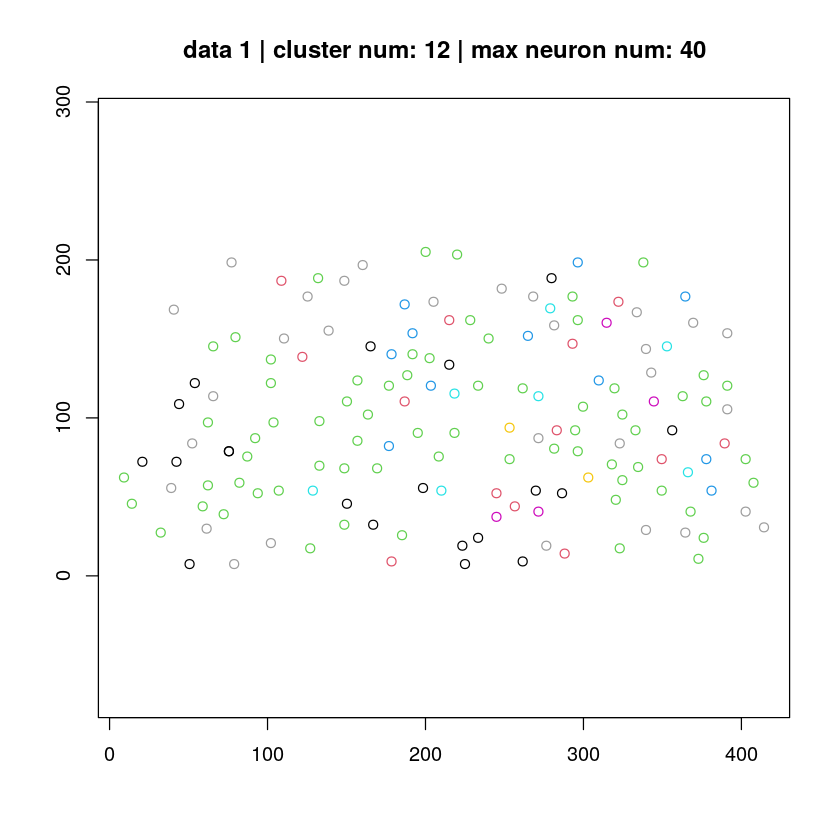
\includegraphics[width=\hsize]{cluster1}
			\end{center}
		\end{minipage}
    \begin{minipage}{0.32\hsize}
			\begin{center}
					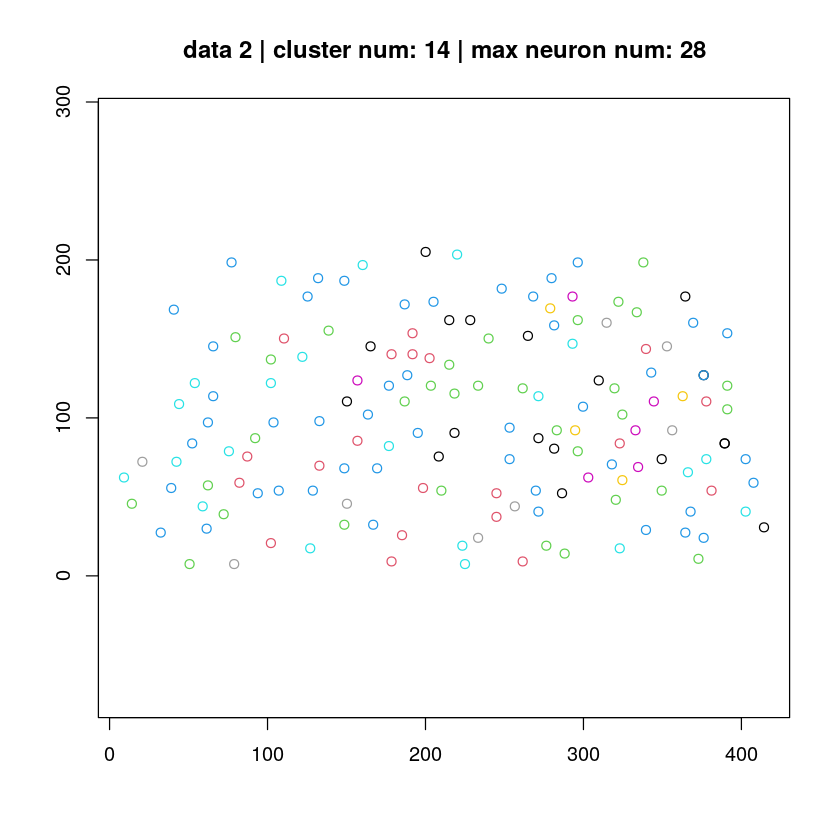
\includegraphics[width=\hsize]{cluster2}
			\end{center}
		\end{minipage}
    \begin{minipage}{0.32\hsize}
			\begin{center}
					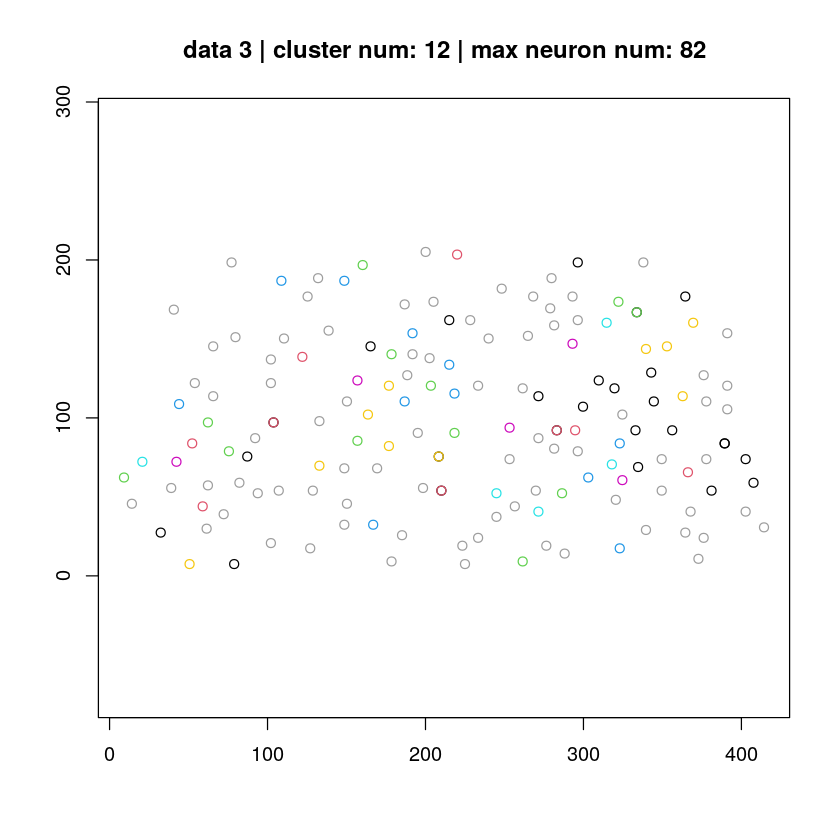
\includegraphics[width=\hsize]{cluster3}
			\end{center}
		\end{minipage}\\
    \begin{minipage}{0.32\hsize}
			\begin{center}
					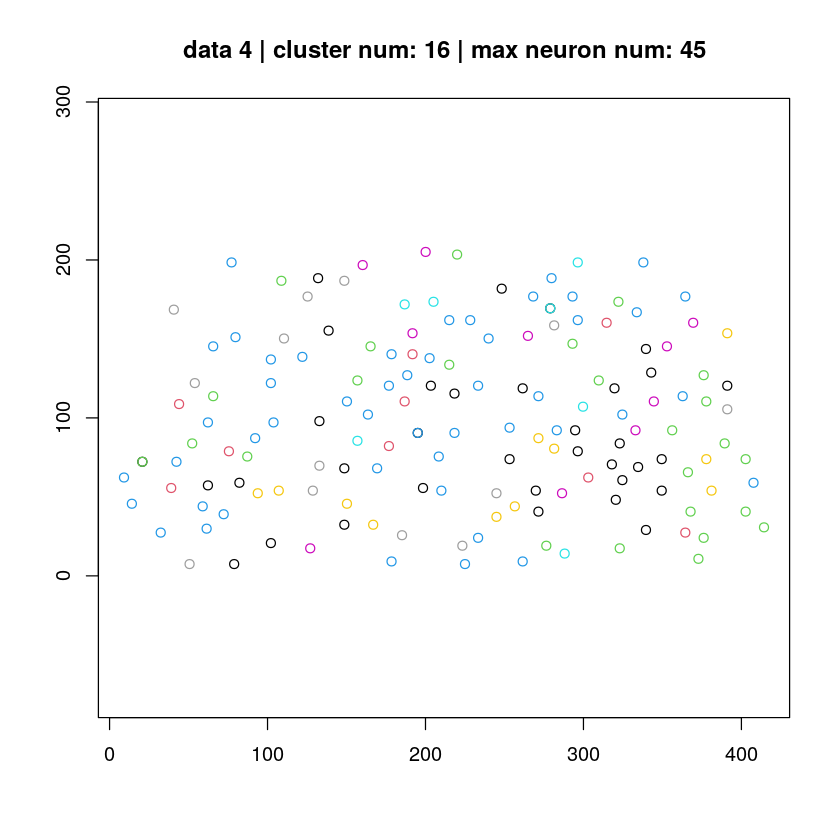
\includegraphics[width=\hsize]{cluster4}
			\end{center}
		\end{minipage}
    \begin{minipage}{0.32\hsize}
			\begin{center}
					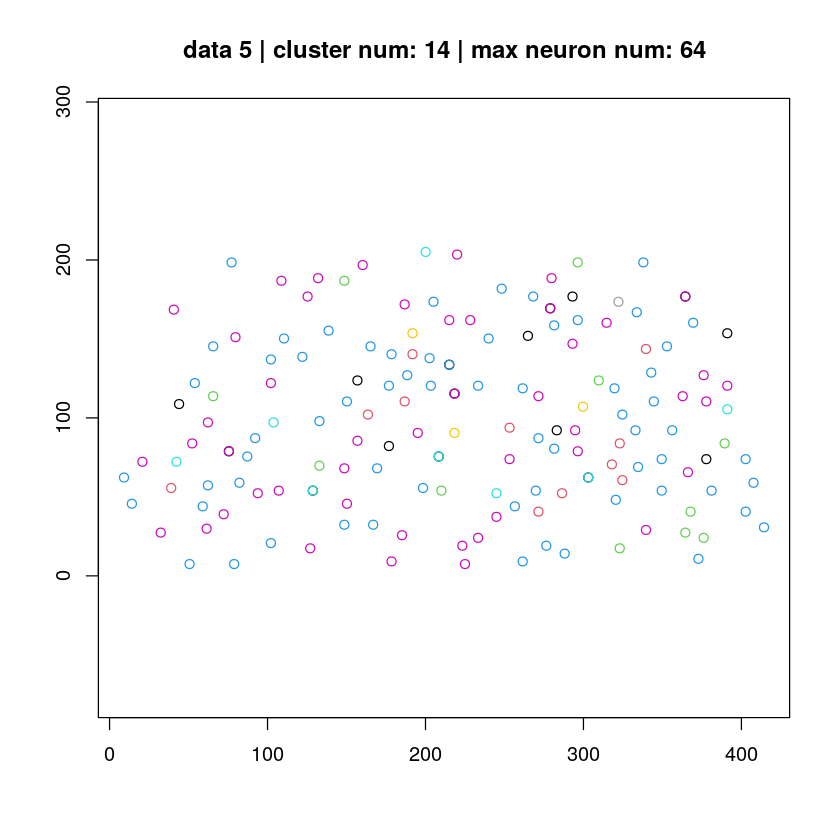
\includegraphics[width=\hsize]{cluster5}
			\end{center}
		\end{minipage}
    \begin{minipage}{0.32\hsize}
			\begin{center}
					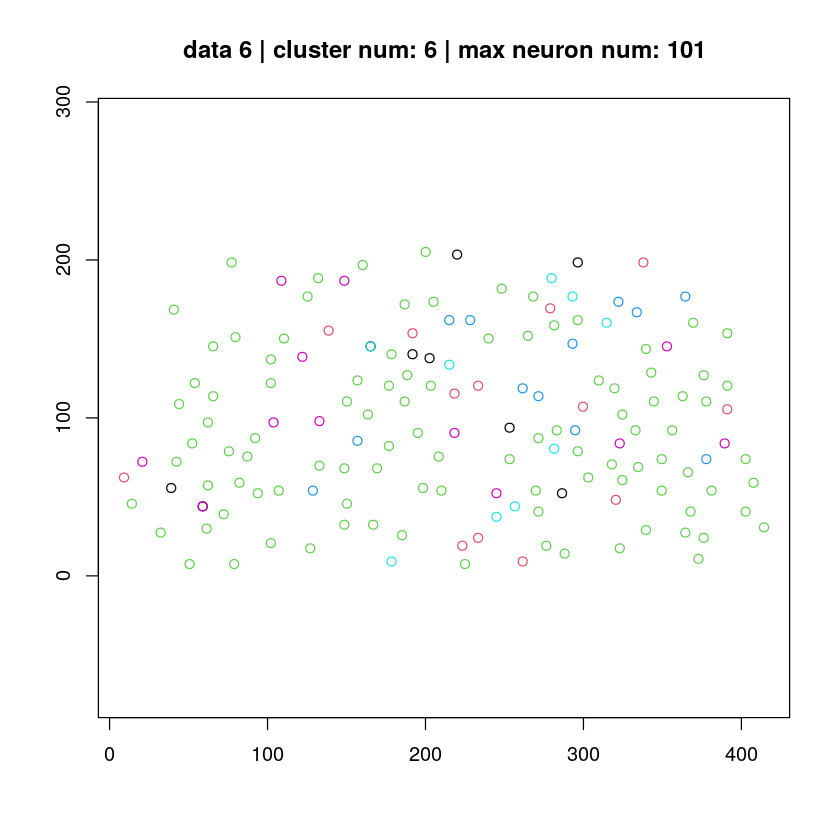
\includegraphics[width=\hsize]{cluster6}
			\end{center}
		\end{minipage}
		\label{fig:real-clst}
\end{figure}

\chapter{結論}
本論文では,サンプリングレートの低いカルシウムイメージングデータからニューロンのクラスタリングを行うことを目的に,ブートストラップ法とNMFを用いた隣接行列推定がクラスタリングに有効であることを確かめた.
データの生成モデルを立てた上で,ニューロン同士の結合推定にNMFを用い,ブートストラップ法をによって結合確率を推定した.
NMFでは基底数を決めることが難しいが,モデル平均によってその問題を緩和した.
提案アプローチが有効であることを人工データ実験によって確かめた.

今後の展望としては,ニューロンが2つのグループに所属する場合にfuzzy clusteringなどが行えるかを確かめる必要がある.
また,第5章で述べた方法でNMFの真の自由度が測れるかどうかも実験を通して確かめたい面白い問題である.

\chapter*{謝辞}
本研究を進めるにあたり指導教員の村田昇先生には多くのご指導をいただきました.
また,今回用いた技術に関する問題の面白さを知ることができました.
深く感謝いたします.
赤穂先生,日野先生,有竹さんにも貴重なお時間を割いて助言をいただき,質問に答えていただきました.
深く感謝いたします.
また,貴重なデータを提供してくださり,カルシウムイメージングやニューロンに関する知見について教えてくださった筑波大学柳沢研究室の上田助教に感謝いたします.

研究室の先輩,同期,後輩にはゼミなどを通じて多くのアドバイスをいただきました.
特に同期の皆様には細かい相談や精神面でも多く支えていただきました.
ありがとうございました.

\backmatter
\begin{otherlanguage}{english}
  % babel-japaneseが若干悪さをするので英語にして回避
  \printbibliography[title=参考文献]
\end{otherlanguage}
\section{補遺}
\subsection{ネットワーク構造のパラメータ値の決め方}
\label{sec:Sparam}
ニューロンのネットワーク構造をsmall world networkによって表すために,初期次数と張り替え確率を実データから決める.
今回はこの値はニューロンのコネクションの割合と相互のコネクションの割合から決める.
興奮性ニューロン同士の6.7\%であり,そのうち双方向のコネクションの割合は24\%である\cite{Jouhanneau2015}.
発達中マウスの興奮性ニューロンから抑制性ニューロンへのコネクティビティと抑制性ニューロンから興奮性ニューロンへのコネクティビティはどちらも78\%であった\cite{Holmgren2003}.
成熟したマウスではより少ないと思われるが,データが見つからなかったため,40\%とした.
相互のコネクションの割合がランダムにエッジを作るよりも高いのは,近いニューロンにコネクションが作られやすいからだと考えられる.
これらのデータを実現するように初期次数と張り替え確率を調整した.
用いたパラメータを\Tabref{tab:parameter1}に示す.
抑制性ニューロン同士のコネクティビティは分からないため,興奮性ニューロンと同じにしている.

\begin{table}[htb]
  \center
  \begin{tabular}{|c|cc|} \hline
    結合の種類 & 初期次数 & 張り替え確率 \\ \hline
		同種類のニューロン間 & $0.0335 N$ & $0.3$ \\
		興奮性ニューロンと抑制性ニューロン間 & $0.2N$ & $0.3$\\ \hline
  \end{tabular}
  \caption{ネットワーク構造のパラメータ値}
  \label{tab:parameter1}
\end{table}

実際のネットワーク構造の作り方を説明する.
ネットワーク構造は興奮性ニューロン同士の結合,抑制性ニューロン同士の結合,興奮性ニューロンと抑制性ニューロン間の結合の3つに分けて作成する.
まず,全ニューロンのうち抑制性ニューロンと興奮性ニューロンのインデックスを決めておく.
全てのニューロンについて\Tabref{tab:parameter1}に従ってネットワークを作成し,それぞれに対応する隣接行列の上三角または下三角行列を取り出して結合する.
作成したいのは向きのある有向グラフなので,上三角行列と下三角行列を分けて作成する.

\subsection{スパイクシミュレーションの設定}
\label{sec:spikeparam}
スパイクシミュレーションで設定しなければならないのは,個々のニューロンの特徴パラメータ,重み付きのネットワーク構造,外部からのランダムな入力である.
これらについて説明する.

まず,個々のニューロンの特徴パラメータについて説明する.
このモデルではニューロンごとに4つのパラメータを設定する必要があり,そのパラメータでニューロンを特徴づける.
本論文では興奮性ニューロンにはregular spiking neurons,抑制性ニューロンにはfast spiking neuronsを用いる.
それらのパラメータを~\Tabref{tab:parameter2}に示す.
ただし,$r_e$と$r_i$は0から1の一様分布に従う確率変数である.

\begin{table}[htb]
  \center
  \begin{tabular}{|c|cccc|} \hline
    ニューロンの種類 & a & b & c & d \\ \hline
    興奮性ニューロン & 0.02 & 0.2 & $-65 + 15 r_e^2$ & $8 - 6r_e^2$ \\
    抑制性ニューロン & $0.02 + 0.08r_i$ & $0.25 - 0.05 r_i$ & -65 & 2 \\ \hline
  \end{tabular}
  \caption{Izhikevichモデルのパラメータ値}
  \label{tab:parameter2}
\end{table}

次に,重み付きのネットワーク構造$W \in \mathbb{R}^{N \times N}$について説明する.
ニューロン$i$から$j$へ結合があった場合,$w_{ij}$はニューロン$i$が発火した時にニューロン$j$の膜電位をどれだけ上昇させるかという数値である.
$W$は,前節で作成した$S$の非ゼロ要素を数値で置き換えることで作成する.
重み付きネットワーク構造$W$の作成方法は2種類ある:
\begin{enumerate}
  \item 全ての重みを同じ分布から生成する
  \item 同じグループへの興奮性ニューロンからの入力は強めにする
\end{enumerate}
1番目の方法では,興奮性ニューロンからの結合は標準偏差$\sigma_w = 1.5$の対数正規分布の$10$以下の分布,抑制性ニューロンからの結合は一様分布$U(-10,0)$からサンプルする.
\begin{align}
	w_{ij} = \begin{cases}
		\{\frac{1}{\sqrt{2 \pi \sigma_w^2}w} \exp \{ - \frac{(\ln w)^2}{2 \sigma_w^2}\} | w \in [0,10]\} & (s_{ij} = 1 \text{,$i$は興奮性ニューロン}) \\
		U(-10,0) & (s_{ij} = 1 \text{,$i$は抑制性ニューロン}) \\
		0 & (s_{ij} = 0)
  \end{cases}
	\label{eq:W}
\end{align}

2番目の方法では,同じグループの興奮性ニューロンからの結合は一様分布$U(7,10)$,異なるグループの興奮性ニューロンからの結合は標準偏差$\sigma_w = 1.5$の対数正規分布の$7$以下の分布,抑制性ニューロンからの結合は一様分布$U(-10,0)$からサンプルする.
対数正規分布を用いる理由は\cite{Song}のデータに基づく.
\begin{align}
	w_{ij} = \begin{cases}
		U(7,10) & (s_{ij} = 1 \text{,$i$は興奮性ニューロン,$i$と$j$は同じグループ}) \\
		\{\frac{1}{\sqrt{2 \pi \sigma_w^2}w} \exp \{ - \frac{(\ln w)^2}{2 \sigma_w^2} \} | w \in [0,7]\} & (s_{ij} = 1 \text{,$i$は興奮性ニューロン,$i$と$j$は異なるグループ}) \\
		U(-10,0) & (s_{ij} = 1 \text{,$i$は抑制性ニューロン}) \\
		0 & (s_{ij} = 0)
  \end{cases}
	\label{eq:W}
\end{align}

最後に外部からのランダムな入力について説明する.
ニューロンには観測範囲外からの入力がある(以降,外部入力とする).
そのため,シミュレーション中も外部からの電位を乱数としてニューロンの電位に足す.
本論文では,ニューロンの活動も外部入力の大きさで表現する.
活動していない興奮性ニューロンと抑制性ニューロンにはそれぞれ,$\mathcal{N}(0,9)$と$\mathcal{N}(0,0.01)$に従う乱数を足す.
活動している興奮性ニューロンと抑制性ニューロンの外部入力は,それぞれの正規分布の平均を$Ne_{plus}$と$Ni_{plus}$とする.
これらを\Tabref{tab:parameter3}に示す.
活動していないニューロンへの外部入力は\cite{Izhikevich2003}で用いられていたものを採用した.
ただし,興奮性ニューロンの活動時の外部入力は変化させた実験もある.

\begin{table}[htb]
  \center
  \begin{tabular}{|c|cc|} \hline
    ニューロンの種類 & 活動時の外部入力 & 活動していない時の外部入力 \\ \hline
		興奮性ニューロン & $\mathcal{N}(Ne_{plus},9)$ & $\mathcal{N}(0, 9)$ \\
		抑制性ニューロン & $\mathcal{N}(Ni_{plus}, 0.01)$ & $\mathcal{N}(0, 0.01)$ \\ \hline
  \end{tabular}
  \caption{シミュレーションに用いる外部入力の値}
  \label{tab:parameter3}
\end{table}

実際の脳でもこのように外部からの入力によってニューロンの活動を制御していると考えられる.
あるニューロングループを活動させる別の方法として,そのグループのハブとなるニューロンにのみ強い外部入力を与える方法も考えられる.

実際のマウスのニューロンの発火頻度を\cite{Watson2016}を元に\Tabref{tab:spike-frequency}に示す.
\Tabref{tab:art_dat}のnon-active120データの興奮性ニューロンと抑制性ニューロンの発火頻度を\Figref{fig:ex_frequency}と\Figref{fig:in_frequency}に示す.
実際のデータと人工データでオーダーは合っていることがわかる.
\Tabref{tab:spike-frequency}のデータは電気生理のデータなので,スパイク頻度の高いニューロンが観測される.
そのため,多少数値が異なっていてもオーダーが合っていれば良いと思われる.
\begin{table}[htb]
  \center
  \begin{tabular}{|c|ccc|} \hline
    ニューロンの種類 & 覚醒時(Hz) & ノンレム睡眠時(Hz) & レム睡眠時(Hz) \\ \hline
		興奮性ニューロン & $0.76 \pm 1.53$ & $0.69 \pm 0.86$ & $0.88 \pm 1.33$ \\
		抑制性ニューロン & $5.59 \pm 7.25$ & $4.69 \pm 5.62$ & $4.25 \pm 9.43$ \\ \hline
  \end{tabular}
  \caption{ニューロンごとの発火頻度の中央値}
  \label{tab:spike-frequency}
\end{table}
\begin{figure}[htbp]
    \begin{minipage}{0.5\hsize}
			\begin{center}
					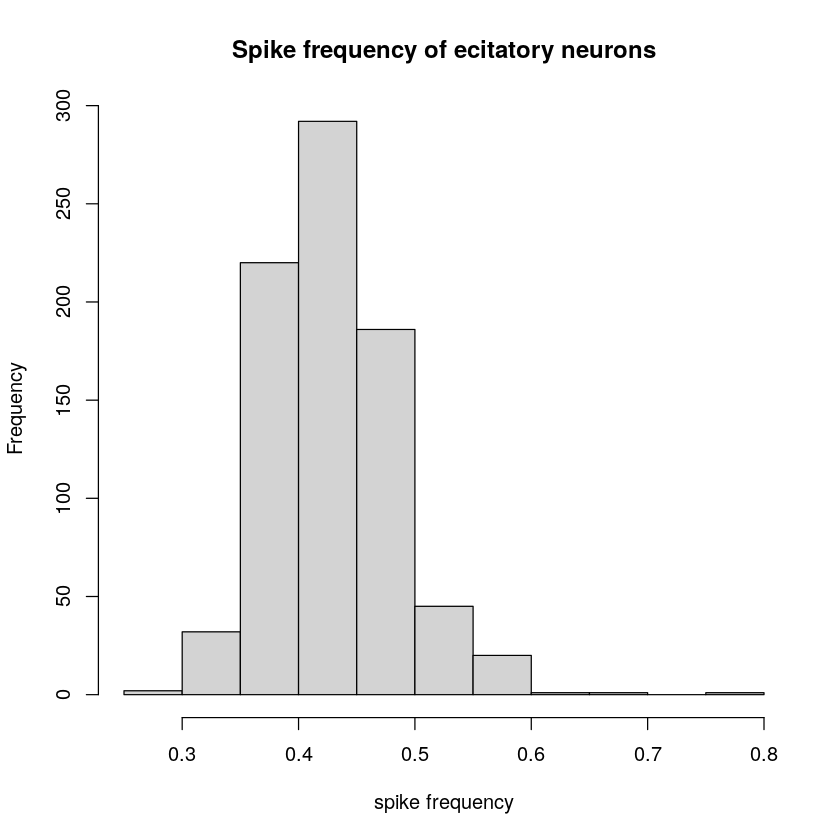
\includegraphics[width=\hsize]{ex_frequency}
					\caption{興奮性ニューロンのスパイク頻度のヒストラグム.}
					\label{fig:ex_frequency}
			\end{center}
		\end{minipage}
    \begin{minipage}{0.5\hsize}
			\begin{center}
					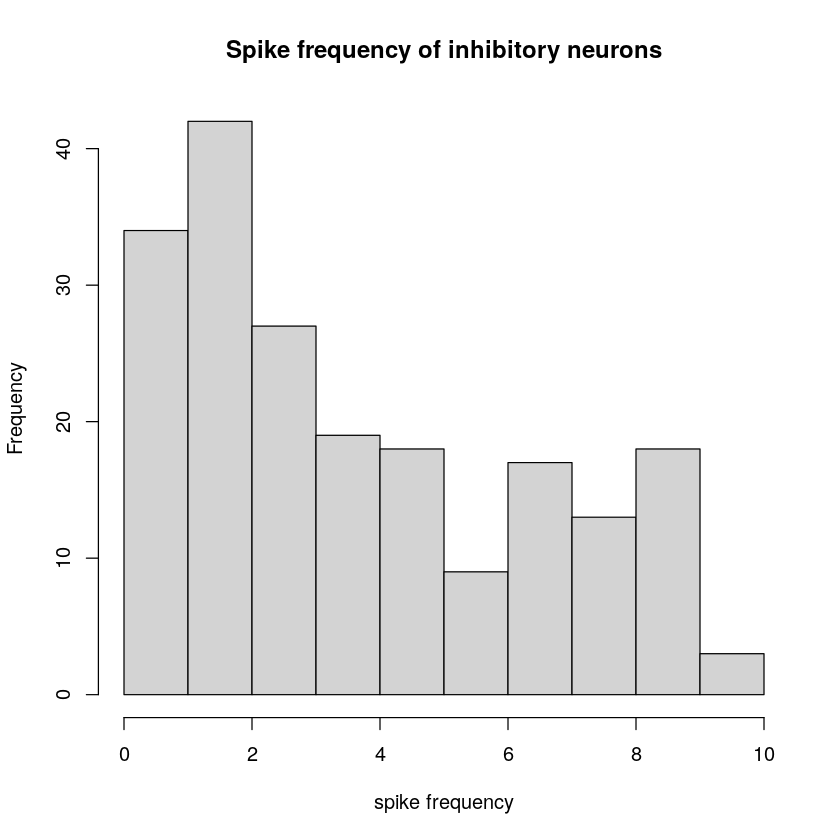
\includegraphics[width=\hsize]{in_frequency}
					\caption{抑制性ニューロンのスパイク頻度のヒストラグム.}
					\label{fig:in_frequency}
			\end{center}
		\end{minipage}
\end{figure}

\chapter{付録A 考案したNMFの制約}
本節では,データの特徴を考慮して考案したNMFの制約とモデルエビデンスの計算方法を紹介する.

% \section{分解能の決定}
% ニューロンの活動データの扱いには時間分解能と空間分解能の2つの側面から検討する必要がある.
% 時間分解能については,蛍光強度データをそのまま用いる,時間窓に区切るなどが考えられる.
% 空間分解能については,ニューロン1個を見る場合,2個を見る場合,複数を見る場合が考えられる.
% 手法によってどのレベルでデータを扱うかが異なる.
% \Tabref{tab:methods}にカルシウムイメージングデータを解析する際に使えそうな手法を載せる.
% これらの手法ではニューロンのネットワーク構造変化やグループの活動の変化などを観察できる.
% 提案アプローチでは行列分解を使いニューロングループを推定し,グループの活動時系列の情報は使わなかった.
% しかし,提案アプローチでも時間窓で区切ってニューロングループの推定を行えばクラスタの変化は抽出できる.
% その際,あまりに短い時間窓内では意味のある情報が取り出せない可能性がある.
% ニューロングループがどれくらいの頻度で活動するのかをある程度の仮定を置いて時間窓を決定する必要がある.
% 
% \begin{table}[htb]
%   \center
%   \begin{tabular}{|c|cc|} \hline
%     & 生データ & 時間窓で区切る \\ \hline
%     ペアで見る & 時系列クラスタリング,TE & glasso,類似度+クラスタリング\\
% 	  複数で見る & 行列分解 & ロジスティック回帰,時系列クラスタリング \\ \hline
%   \end{tabular}
%   \caption{カルシウムイメージングデータ解析に使えそうな手法}
%   \label{tab:methods}
% \end{table}
% 
\section{スケール除去}
ニューロンごとに発現している蛍光タンパク質の量や細胞の大きさが異なる.
そのため,ニューロンごとのバイアスが観測データに載っていると考え,バイアスを除去する方法を試した.
この時の数理モデルは以下のようになる:
\begin{equation}
	X = DC + H + B.
\end{equation}
ただし,$B \in \mathbb{R}_+^{I\times J}$は行ごとに同じ数値が入ったバイアス行列である.

バイアスの推定方法は,$D$に1列を足し,$C$に$\mathbf 1$の1行を足してNMFを更新する.
$D$の列にバイアスが推定されることを期待した.

簡単な人工データ実験を行った結果,足したバイアスよりも大きいバイアスが推定されてしまうことがわかった.
また,そもそもの数理モデルが異なると考え直した.

蛍光タンパク質の量や細胞の大きさが異なるということは,各ニューロンはスケールされていると考えられ,以下のように表される:
\begin{equation}
	X = A(DC + H).
\end{equation}
ただし,$A \in \mathbb{R}_+^{I \times I}$は対角行列である.

ナイーブな求め方は,$A$は単位行列で初期化し,NMF一回の更新ごとに$X$をニューロンごとに残差の四分位範囲で割り,その値を$A$にかけていく.
簡単な人工データ実験で乗法更新則を用いた場合は$A$は真の値に近いものが推定された.

\section{重複除去}
本研究で置いた仮定では,あるニューロンが複数のグループに所属する時,グループの活動は被らないとしている.
しかし,NMFの推定時にそのような制約は入れていないので,NMFで推定した結果この仮定が破られているようであれば制約は入れなければならない.

そこで,以下の目的関数を考えた:
\begin{align}
	\argmin_{D \geq 0, C \geq 0} ||X - DC||_F^2 - \lambda \sum_{k=1}^K \sum_{l \neq k}^K \left( || d_{:l} - d_{:k} ||_1 || c_{l:} - c_{k:} ||_1 \right).
  \label{eq:overlap}
\end{align}

更新則を導出する.
参考にしたのは\cite{Babaee2016}である.
\eqref{eq:overlap}のLagrange関数$L$は,
\begin{align}
	L = &\text{Tr}(X^TX) - 2 \text{Tr}(X^TDC) + \text{Tr}(C^TD^TDC) - \text{Tr}(\Phi_C C^T)\\
	&- \text{Tr}(\Phi_D D^T) - \lambda \text{Tr} (F^T C H^T S^T D F),
\end{align}
であり,KKT条件は,
\begin{align}
	\frac{\partial L}{\partial C} = \frac{\partial L}{\partial D} = 0 \\
	D \geq 0 \\
	C \geq 0 \\
	\Phi_C \geq 0 \\
	\Phi_D \geq 0 \\
	\Phi_C C = \Phi_D D = 0
\end{align}
である.
ただし,$\Phi_D$と$\Phi_C$はそれぞれ$D \geq 0$,$C \geq 0$に対するLagrange乗数で,$F \in [0,1]^{K \times (K-1)!}$は2つの時間の組み合わせを表現した以下のような行列である:
\begin{equation}
	F = \left(
    \begin{array}{cccccc}
			1 & 1 & \ldots & 0 & \ldots & 0 \\
			-1 & 0 & \ldots & 1 & \ldots & 0 \\
			0 & -1 & \ldots & -1 & \ldots & 0 \\
			\vdots & \vdots & \vdots & \vdots & \ddots & \vdots \\
			0 & 0 & \ldots & 0 & \ldots & 1 \\
			0 & 0 & \ldots & 0 & \ldots & -1
    \end{array}
  \right).
\end{equation}
また,$S = sign(DF)$,$H = sign(F^TC)$とおく.

$D$を求めるには以下の式を解く:
\begin{equation}
	\frac{\partial L}{\partial D} = - 2 X C^T + 2 DCC^T - \Phi_D - \lambda SHC^T FF^T = 0.
\end{equation}
これを求めると$D$の要素の更新は以下である:
\begin{equation}
	d_{ik} \leftarrow d_{ik} \frac{2[XC^T]_{ik} + \lambda [SHC^T FF^T]_{ik}^+}{2[DCC^T]_{ik} - \lambda [SHC^T FF^T]_{ik}^-}.
\end{equation}
ただし,$[\cdot]^+$は行列の中の正の要素,$[\cdot]^-$は負の要素である.

同様に,$C$の要素の更新は以下の通りである:
\begin{equation}
	c_{kj} \leftarrow c_{kj} \frac{2[D^T X]_{kj} + \lambda [FF^T D^T SH]_{kj}^+}{2[D^T DC]_{kj} - \lambda [FF^T D^T SH]_{kj}^-}.
\end{equation}

しかし,ハイパーパラメータ$\lambda$の最適な決め方は分からない.
また,$\lambda$が大きいと$D$と$C$はスパースになるが,本来2つの基底に所属するニューロンの$d_{i:}$が1つの基底以外0に近くなることが実験を通してわかった.
この手法は改善の余地がある上,実際のデータをNMFで分解した際にどれくらい仮定に沿っていないかを確認した上で使う必要がある.

\section{時間方向への制約}
カルシウムイメージングデータはスパイク情報を反映するのが遅く,一度上がった蛍光強度は緩やかに下がっていく.
そのため,NMFで分解を行う際も,行列$C$の時間方向に前時刻の値と近くなるような制約を入れることでより正確なニューロングループの抽出が行えると考えられる.
$C$の偶数列を前後の列の平均とするNMFも提案されている~\cite{Cheung2015}.
しかし,これはかなりスムースになる制約だと考えられる.
そこで,以下のような制約を加えた目的関数が考えられる:
\begin{equation}
	\argmin_{D \geq 0, C \geq 0}||X - DC||^2_F + \lambda \sum_t||c_{:t} - c_{:t-1}||_1.
  \label{eq:NMF-ar}
\end{equation}
これはfused lasso \cite{Tibshirani2005}と同じような制約である.

更新則は,$D$は\eqref{eq:nmf_fro}と同じだが$C$は異なり以下である:
\begin{equation}
	c_{kj} \leftarrow c_{kj} \frac{2[D^T X]_{kj} - s_{kj}}{2[D^T DC]_{kj}}.
\end{equation}
ただし,$s_{:j} = sign(c_{:j} - c_{:j-1})$であり,1列目のみ$s_{:1} = \mathbf{0}$である.

重複除去制約と同じく,$\lambda$の決め方が分からないため使用は断念した.
NMFは初期値依存の問題があるため,$\lambda$を変化させると解空間も変化し,結果は滑らかに変化しない.
そのため,$\lambda$を変化させた効果を比較するのは難しい.

\chapter{付録B NMFのモデルエビデンス}
NMFの基底数を決める際にブートストラップから計算されたモデルエビデンスを用いることを考える.
BICは最尤推定量の尤度からモデルエビデンスを近似して扱っている.
モデルエビデンスはブートストラップ法によっても近似計算できると考えられる.

基底数$k$のNMFのモデルを$\mathcal{M}_k$とおく.
ノイズ行列$H$の各要素が正規分布$\mathcal{N} (0, \sigma^2)$に従う$\mathcal{M}_k$の尤度は以下である:
\begin{align}
	p(X | Y_k, \mathcal{M}_k) = \prod_{i,j} \frac{1}{\sqrt{2 \pi \sigma^2}} \exp(-\frac{([Y_k]_{ij} - x_{ij})^2}{2 \sigma^2}).
	\label{eq:likelihood}
\end{align}
ただし,$Y_k = D_k C_k$で,$Y_k$はモデル$\mathcal{M}_k$における推定量である.
対数尤度は以下のようになる.
\begin{align}
	\log p(X | Y_k, \mathcal{M}_k) = - \frac{IJ}{2} (\log 2\pi + 2 \log \sigma) - \frac{1}{2 \sigma^2} \sum_{ij}([Y_k]_{ij} - x_{ij})^2.
\end{align}

今回の問題をBayesian model averagingの枠組みに当てはめると,異なる基底数のNMFから求まった$\bar{A}$をモデルの事後確率で重み付て足し合わせることになる.
この時の式は,
\begin{align}
	p(\bar{A}|X) = \sum_k p(\bar{A}|\mathcal{M}_k, X) p(\mathcal{M}_k | X),
\end{align}
で$p(\bar{A}|X)$を求めることになる.

モデルの事後確率は
\begin{align}
	p(\mathcal{M}_k|X) = \frac{m_k p(\mathcal{M}_k)}{\sum_l m_l p(M_l)},
\end{align}
で表される.
ただし,
\begin{align}
	m_k = \int p(X | Y_k, \mathcal{M}_k) p(Y_k| \mathcal{M}_k) dY_k,
	\label{eq:evidence}
\end{align}
である.
これはモデルエビデンスやmarginal likelihoodと呼ばれる.
また,$p(\mathcal{M}_k)$はモデルが正しい確率である.

ある条件下で,母数の事後確率の密度関数はブートストラップによる最尤推定量の分布と同じになる.
そのため,ブートストラップサンプルから推定した$Y_k$の分布をもとに事後確率を計算すれば良い.

現在は$p(\mathcal{M}_k)$に関する知識はなく無情報なため,モデルエビデンスを推定することで各モデルの重みが求まる.

\section{ラプラス近似}
モデルエビデンスの計算には事前分布を決めなければならず,積分も計算しなければいけない.
そこでラプラス近似により$m_k$は以下のような$\hat{m_k}$で近似できる.
\begin{align}
	\log \hat{m}_k = \log p(X | \hat{Y_k}, \mathcal{M}_k) - \frac{d_k}{2} \log n.
	\label{eq:simm}
\end{align}
ここで,$d_k$は母数の数($I \times K + K \times J$),$n$は観測データ数($J$)である.
この近似を使ってBayes因子のログをとったものがBICである.
Bayes因子は2つのモデルエビデンスの比である.
NMFではデータの増加とともにパラメータ数も増加するため,BICを用いて基底数を決めるのは本来適さない.

実験では,$\log p(X | \hat{Y_k}, \mathcal{M}_k)$は初期値を変えてNMFを行い,尤度が最も大きくなった対数尤度を用いる.
また,$\sigma^2 = Var(X - Y_k)$として計算する.

\section{ブートストラップによる近似}
ブートストラップの推定量の分布は最尤推定量の分布を近似する(ブートストラップサンプルが生成されたパラメータ分バイアスは乗る).
これを簡単なデモンストレーションで確認する.

人工的に$D$と$C$を作成し,標準正規分布に従うノイズを加えて$X$を作る.
事後確率$p(\mathcal{M}_k | X)$は
\begin{align}
	p(\mathcal{M}_k | X) &= \frac{p(X | Y_k, \mathcal{M}_k) p(\mathcal{M}_k)}{p(X)},
\end{align}
である.
事前分布$p(\mathcal{M}_k)$を無情報とした時,事後確率は尤度に比例する.
そこで,データ$X$のある2要素$(i,j)$と$(i',j')$について尤度の分布を図示する.
ノイズに標準正規分布を用いたので,$\sigma = 1$として\eqref{eq:likelihood}を2つの要素のある範囲について計算する.
求めたいのは事後確率の分布なので,「$[Y_k]_{ij}=5$かつ$[Y_k]_{i'j'}=8$の時の尤度を計算する」ことを5や8の値をずらしながら行う.
その結果を\Figref{fig:posprob}に示す.
\begin{figure}[htbp]
    \begin{minipage}{0.5\hsize}
			\begin{center}
					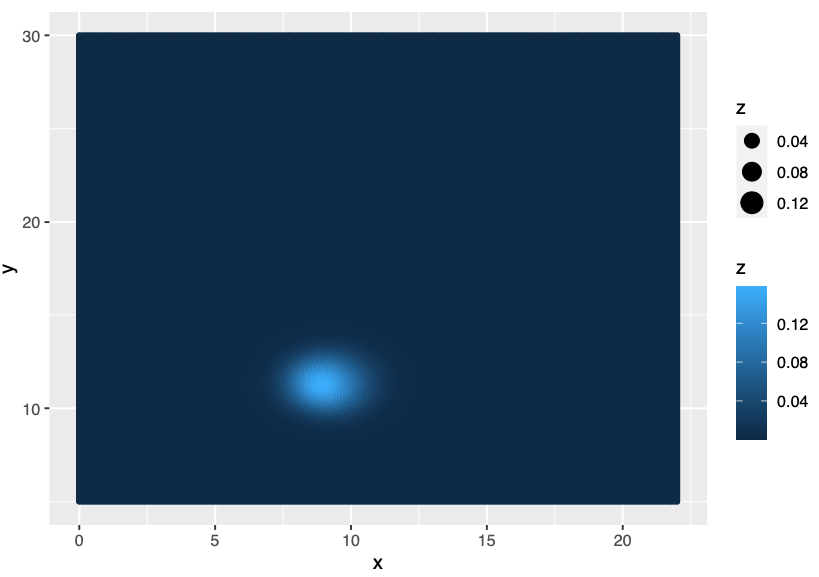
\includegraphics[width=\hsize]{posterior_prob}
					\caption{人工データの2つの要素の尤度分布}
					\label{fig:posprob}
			\end{center}
		\end{minipage}
    \begin{minipage}{0.5\hsize}
			\begin{center}
					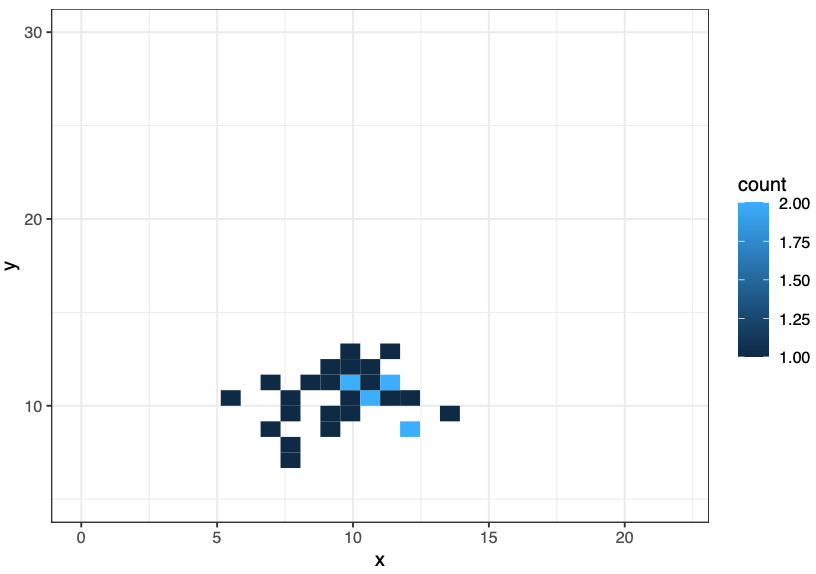
\includegraphics[width=\hsize]{boot_prob30}
					\caption{30個のブートストラップサンプルから推定された2つの要素の値の分布}
					\label{fig:boot_prob30}
			\end{center}
		\end{minipage}\\
    \begin{minipage}{0.5\hsize}
			\begin{center}
					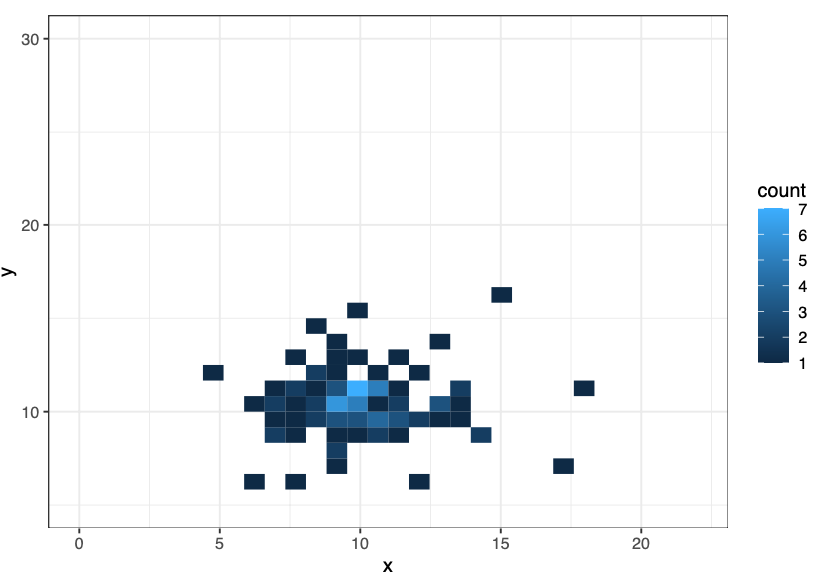
\includegraphics[width=\hsize]{boot_prob100}
					\caption{100個のブートストラップサンプルから推定された2つの要素の値の分布}
					\label{fig:boot_prob100}
			\end{center}
		\end{minipage}
    \begin{minipage}{0.5\hsize}
			\begin{center}
					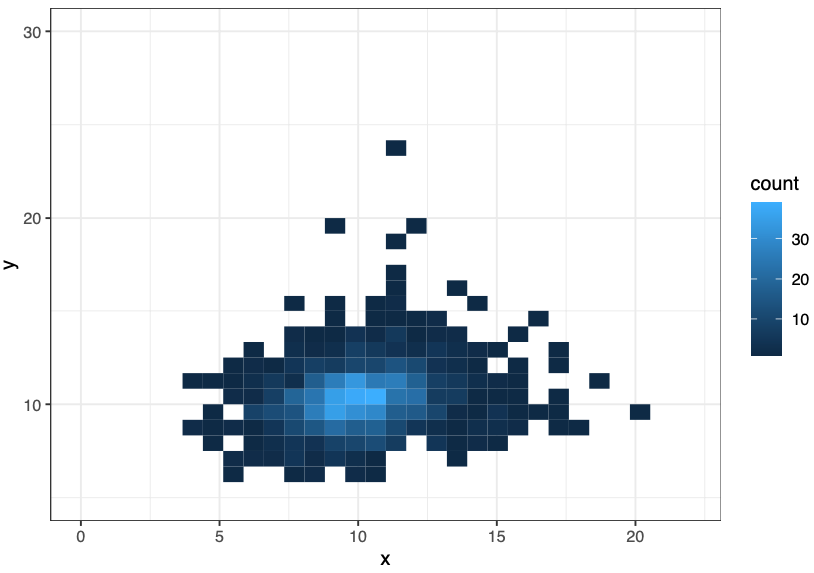
\includegraphics[width=\hsize]{boot_prob1000}
					\caption{1000個のブートストラップサンプルから推定された2つの要素の値の分布}
					\label{fig:boot_prob1000}
			\end{center}
		\end{minipage}
\end{figure}

次に,ブートストラップの推定量が\Figref{fig:posprob}を近似することを確かめる.
ブートストラップサンプルを作成しNMFを行い,\Figref{fig:posprob}の2要素についてヒートマップを作成する.
その結果をブートストラップのサンプル数別に\Figref{fig:boot_prob30}〜\ref{fig:boot_prob1000}に示す.
これより,\Figref{fig:boot_prob1000}は\Figref{fig:posprob}の分布を近似できていることがわかる.

これより,ブートストラップの推定量の分布は最尤推定量の分布を近似するので,$m_k$は以下のように近似できる.

\begin{align}
	m_k &= \int p(X | Y_k, \mathcal{M}_k) p(Y_k| \mathcal{M}_k) dY_k \\
	&\sim \frac{1}{B} \sum_b \prod_{i,j} \frac{1}{\sqrt{2 \pi \sigma^2}} \exp\left(-\frac{([Y_k^b]_{ij} - X^b_{ij})^2}{2 \sigma^2} \right).
	\label{eq:simm2}
\end{align}

ここで,$Y_k^b$はブートストラップサンプル$b$から計算された$Y_k$で,$B$はブートストラップサンプル数である.
また,$\sigma^2 = Var(X^b - Y^b_k)$として計算する.

\section{実験}
人工データセット86個について2つの近似方法でモデルエビデンスを計算した.
その結果を\Figref{fig:evidence1}と\Figref{fig:evidence2}に示す.
同じデータの結果を線で結んでいる.
ラプラス近似を行った場合は真の基底数10付近で最大値をとっている.
ブートストラップによる近似を行った場合は基底数に比例してモデルエビデンスの値も大きくなっている.
また,同じデータでも基底数によってオーダーが大きく異なるが,これは尤度計算に用いる分散をデータから計算しているためである.

\begin{figure}[htbp]
    \begin{minipage}{0.5\hsize}
			\begin{center}
					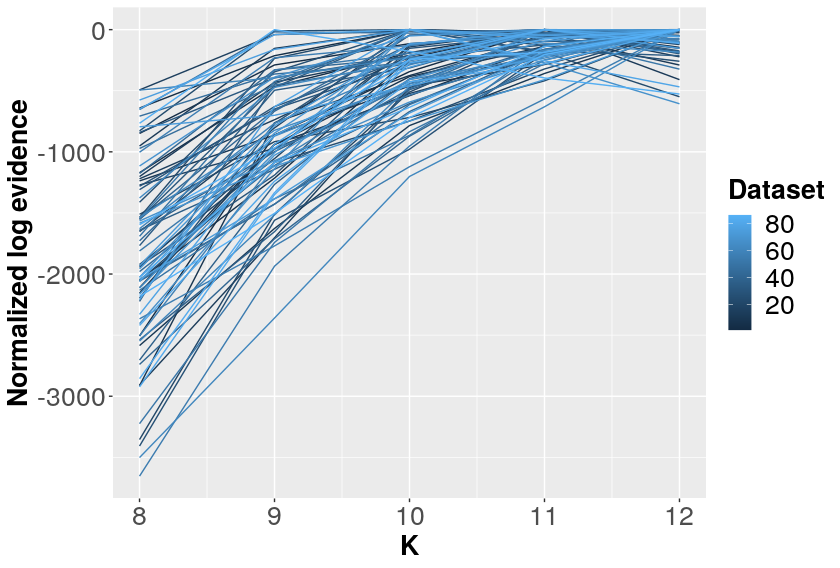
\includegraphics[width=\hsize]{evidence1log}
					\caption{ラプラス近似によって計算されたログエビデンス.各データについて最大値が0となるように定数を足した.}
					\label{fig:evidence1}
			\end{center}
		\end{minipage}
    \begin{minipage}{0.5\hsize}
			\begin{center}
					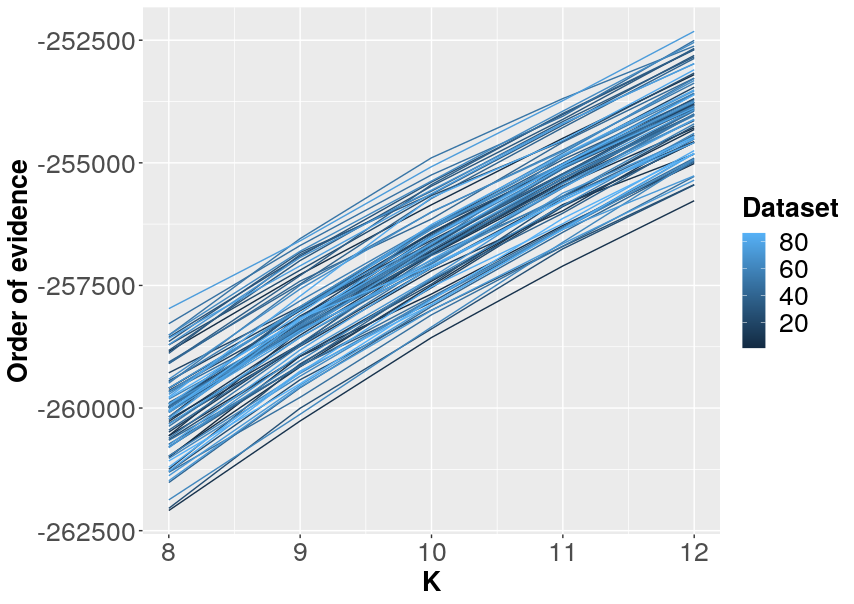
\includegraphics[width=\hsize]{evidence2order}
					\caption{ブートストラップ近似によって計算されたエビデンスのオーダー(10を底とした指数).}
					\label{fig:evidence2}
			\end{center}
		\end{minipage}
\end{figure}

また,\Figref{fig:evidence2}のログを取り,\Figref{fig:evidence1}とプロットした図を\Figref{fig:evidence12}に示す.
これより,ブートストラップによる近似を用いた場合のモデルエビデンスの値は大きいことが分かる.
ラプラス近似では$\frac{d_k}{2} \log n$というパラメータ数による補正が加わっているため,ブートストラップによるモデルエビデンスの方が高い値を持つ.
逆に,\Figref{fig:evidence12}の2つの近似手法のモデルエビデンスの差が過剰に足された補正の値だと考えることもできる.
つまり,$\frac{d_k}{2} \log n$から2つのモデルエビデンスの差を引いた数値がNMFの真の自由度であるとも考えられる.
これを確かめるためには数値実験を行う必要がある.

\begin{figure}[htbp]
    \begin{center}
        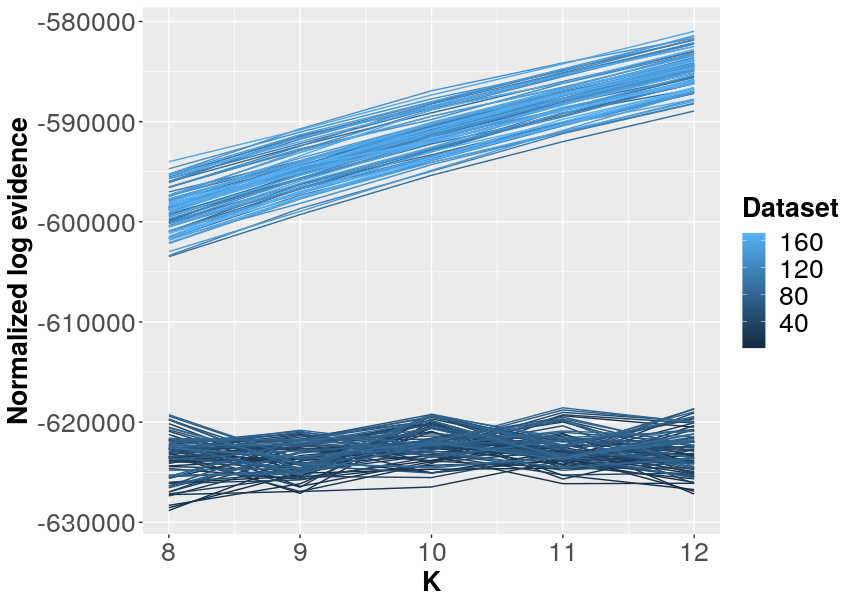
\includegraphics[width=0.8\linewidth]{evidence12log}
        \caption{2つの近似方法によって計算されたログエビデンス.}
        \label{fig:evidence12}
    \end{center}
\end{figure}

\end{document}
